% ============================================================
% main.tex
% ANSpect O-EMA · MS Thesis · UTD Electrical Engineering
% Compiler: pdflatex · Class: utdthesis.cls
% Style: IEEEtran (natbib numbers mode)
% ------------------------------------------------------------
% CHANGELOG
% v1.0  27-Aug-2026  Initial baseline
% v1.1  01-Sep-2026  Split chapters.tex → 5 separate chapter files
%                    Added \setcounter{tocdepth}{3}
%                    Added pdfborder={0 0 0} to hyperref
%                    Added \raggedbottom
%                    Updated author, prevdegrees, committeemember*
%                    Updated \degreefull to Master of Science
%                    Updated \title with \texttrademark{}
% v1.2  01-Sep-2026  Added conservative display skip adjustments
%                    to reduce excess equation spacing (8pt values)
%                    Verified: no UTD rule violation, no forbidden
%                    package, compatible with \flushbottom
% v1.3  02-Sep-2026  Added glossaries pkg (Option B) for List of Abbreviations
%                    Auto-collect from \gls{} in text · auto-sort · no page numbers
%                    TOC entry auto-generated · first-use expansion enabled
%                    abbrevs.tex → separate definitions file
%                    glossaries loads AFTER hyperref (pkg requirement — not a UTD violation)
% v1.4  02-Sep-2026  Removed toc option from glossaries pkg
%                    utdthesis.cls auto-generates TOC entry — toc option caused duplicate
% ============================================================

\documentclass[doublespacing]{utdthesis}

% ------------------------------------------------------------
% PACKAGES
% FORBIDDEN (UTD_RULES.md): geometry · setspace ·
%   font-size overrides · caption style overrides ·
%   chapter heading overrides · TOC/LOF/LOT overrides
% ------------------------------------------------------------
\usepackage{amsmath}
\usepackage{amssymb}
\usepackage{graphicx}
\usepackage{url}
\usepackage{microtype}
\usepackage{rotating}           % sidewaystable only
\usepackage[numbers]{natbib}
\bibliographystyle{IEEEtran}
\setcounter{tocdepth}{3}

% ------------------------------------------------------------
% EQUATION DISPLAY SPACING
% Reduces excess vertical space around display equations
% caused by utdthesis.cls doublespacing mode.
% v1.2  01-Sep-2026  Added — conservative 8pt values
% UTD compliance: not a forbidden package, no line-spacing
%                 override, compatible with \flushbottom
% ------------------------------------------------------------
\setlength{\abovedisplayskip}{8pt plus 2pt minus 2pt}
\setlength{\belowdisplayskip}{8pt plus 2pt minus 2pt}
\setlength{\abovedisplayshortskip}{4pt plus 2pt}
\setlength{\belowdisplayshortskip}{4pt plus 2pt}

% hyperref — always last before acronym
\usepackage[pdftex,bookmarks,colorlinks=false,pdfborder={0 0 0}]{hyperref}

% acronym — List of Abbreviations
% Single-pass · no makeglossaries · no external tools
% \acro{label}[SHORT]{Long Form}  defined in abbrevs.tex
% \ac{label}  → "Long Form (SHORT)" first use, "SHORT" thereafter
% \acp{label} → plural (appends -s to SHORT)
\usepackage{acronym}

% ------------------------------------------------------------
% THESIS METADATA — fill all [PENDING] before submission
% ------------------------------------------------------------
\author{Sathwik Sudhindranath}
\title{RFSoC 4x2 FPGA Implementation ANSpect O-EMA\texttrademark{} j.83B Tx/Rx [NDA-TITLE]}
\thesistype{Thesis}
\degreefull{Master of Science}
\degreeabbr{MS}
\subject{Electrical Engineering}
\graduationmonth{December}
\graduationyear{2026}
\prevdegrees{B.E., Electronics \& Communication Engineering,
  Visvesvaraya Technological University, 2021}
\committeemember*{Dr.\ Benjamin Carrion Schaefer}
\committeemember{[MEMBER 2 PENDING]}
\committeemember{[MEMBER 3 PENDING]}

% ============================================================
\begin{document}
% ============================================================

% ------------------------------------------------------------
% FRONTMATTER — roman numeral pagination
% Page count order per UTD_RULES.md:
%   First Page · Copyright · (Dedication) · Title ·
%   Acknowledgments · Abstract · TOC · LOF · LOT ·
%   (List of Abbreviations)
% ------------------------------------------------------------
\frontmatter

\signaturepage           % First Page (formerly signature page)
\copyrightpage{2026}     % recommended — year = conferral year

% Dedication — optional; uncomment when ready
% \begin{dedication}
%   % TODO: dedication text
% \end{dedication}

\maketitle               % Title Page

\begin{acks}{December 2026}
  % TODO: Acknowledgments — complete sentences and paragraphs
  % No \section commands inside acks environment
\end{acks}

\begin{abstract}
  % TODO: ≤500 words — continuous prose — no bullets
  % Run 'word count abstract [tex]' before submission
  % Title must match title page exactly
  % Author name must match all other pages
\end{abstract}

\tableofcontents
\listoffigures           % required: ≥5 figures expected
\listoftables            % required: ≥5 tables expected

% List of Abbreviations — built from abbrevs.tex
% Single pdflatex pass · no makeglossaries required
% utdthesis.cls styles \chapter* heading; TOC entry added manually
\phantomsection
\addcontentsline{toc}{chapter}{List of Abbreviations}
\chapter*{List of Abbreviations}
\begin{acronym}[MPEG-TS]   % longest SHORT label sets column width
  % ============================================================
% abbrevs.tex
% ANSpect O-EMA · MS Thesis · UTD Electrical Engineering
% Package: acronym (replaces glossaries — v1.2)
% Usage in text:  \ac{label}   → first use: Long Form (SHORT)
%                              → thereafter: SHORT
%                 \acp{label}  → plural SHORT (appends s)
%                 \Ac{label}   → capitalised long form on first use
% List prints via \begin{acronym}[MPEG-TS]% ============================================================
% abbrevs.tex
% ANSpect O-EMA · MS Thesis · UTD Electrical Engineering
% Package: acronym (replaces glossaries — v1.2)
% Usage in text:  \ac{label}   → first use: Long Form (SHORT)
%                              → thereafter: SHORT
%                 \acp{label}  → plural SHORT (appends s)
%                 \Ac{label}   → capitalised long form on first use
% List prints via \begin{acronym}[MPEG-TS]% ============================================================
% abbrevs.tex
% ANSpect O-EMA · MS Thesis · UTD Electrical Engineering
% Package: acronym (replaces glossaries — v1.2)
% Usage in text:  \ac{label}   → first use: Long Form (SHORT)
%                              → thereafter: SHORT
%                 \acp{label}  → plural SHORT (appends s)
%                 \Ac{label}   → capitalised long form on first use
% List prints via \begin{acronym}[MPEG-TS]\input{abbrevs}\end{acronym}
%   in main.tex frontmatter — no makeglossaries needed.
% ------------------------------------------------------------
% CHANGELOG
% v1.0  02-Sep-2026  Initial — glossaries \newacronym format
% v1.1  02-Sep-2026  Confirmed working with glossaries Option B
% v1.2  24-Sep-2026  REFORMAT: glossaries → acronym pkg
%                    All \newacronym → \acro
%                    Sorted A→Z by SHORT form (256-QAM under Q)
%                    CH-1, CH-4, CH-5 entries: TODO before draft
% ============================================================

% ------------------------------------------------------------
% A
% ------------------------------------------------------------
\acro{adc}[ADC]{Analog-to-Digital Converter}
\acro{amba}[AMBA]{Advanced Microcontroller Bus Architecture}
\acro{api}[API]{Application Programming Interface}
\acro{apu}[APU]{Application Processing Unit}
\acro{arm}[ARM]{Advanced RISC Machine}
\acro{asic}[ASIC]{Application-Specific Integrated Circuit}
\acro{axi}[AXI]{Advanced eXtensible Interface}

% ------------------------------------------------------------
% B
% ------------------------------------------------------------
\acro{bcc}[BCC]{Binary Convolutional Code}
\acro{bram}[BRAM]{Block Random-Access Memory}

% ------------------------------------------------------------
% C
% ------------------------------------------------------------
\acro{clb}[CLB]{Configurable Logic Block}
\acro{cmts}[CMTS]{Cable Modem Termination System}
\acro{cpe}[CPE]{Customer Premises Equipment}
\acro{cpu}[CPU]{Central Processing Unit}
\acro{cl}[CL]{Configurable Logic}
\acro{crc}[CRC]{Cyclic Redundancy Check}

% ------------------------------------------------------------
% D
% ------------------------------------------------------------
\acro{dac}[DAC]{Digital-to-Analog Converter}
\acro{ddc}[DDC]{Digital Down-Converter}
\acro{ddr}[DDR]{Double Data Rate}
\acro{dma}[DMA]{Direct Memory Access}
\acro{docsis}[DOCSIS]{Data Over Cable Service Interface Specification}
\acro{dsp}[DSP]{Digital Signal Processing}
\acro{duc}[DUC]{Digital Up-Converter}
\acro{dpt}[DPT]{Differential Precoder Table}

% ------------------------------------------------------------
% E
% ------------------------------------------------------------
\acro{evm}[EVM]{Error Vector Magnitude}

% ------------------------------------------------------------
% F
% ------------------------------------------------------------
\acro{fec}[FEC]{Forward Error Correction}
\acro{ff}[FF]{Flip-Flop}
\acro{fifo}[FIFO]{First-In First-Out}
\acro{fir}[FIR]{Finite Impulse Response}
\acro{fpga}[FPGA]{Field-Programmable Gate Array}
\acro{fsm}[FSM]{Finite State Machine}

% ------------------------------------------------------------
% G
% ------------------------------------------------------------
\acro{gsps}[GSPS]{Giga-Samples Per Second}
\acro{gf}[GF]{Galois Field}

% ------------------------------------------------------------
% H
% ------------------------------------------------------------
\acro{hfc}[HFC]{Hybrid Fiber-Coaxial}
\acro{hp}[HP]{High-Performance}
% under % H, after \acro{hp}:
\acro{hdl}[HDL]{Hardware Description Language}

% ------------------------------------------------------------
% I
% ------------------------------------------------------------
\acro{ip}[IP]{Intellectual Property}
\acro{iq}[IQ]{In-Phase/Quadrature}
\acro{isi}[ISI]{Inter-Symbol Interference}
\acro{itut}[ITU-T]{International Telecommunication Union -- Telecommunication Standardization Sector}

% ------------------------------------------------------------
% L
% ------------------------------------------------------------
\acro{ldpc}[LDPC]{Low-Density Parity-Check}
\acro{lfsr}[LFSR]{Linear Feedback Shift Register}
\acro{lsb}[LSB]{Least Significant Bit}
\acro{lut}[LUT]{Look-Up Table}
\acro{lut6}[LUT6]{Six-Input Look-Up Table}
\acro{led}[LED]{Light-Emitting Diode}

% ------------------------------------------------------------
% M
% ------------------------------------------------------------
\acro{mac}[MAC]{Multiply-Accumulate}
\acro{mm}[MM]{Memory-Mapped}
\acro{mm2s}[MM2S]{Memory-Mapped to Stream}
\acro{mpegts}[MPEG-TS]{MPEG Transport Stream}
\acro{msb}[MSB]{Most Significant Bit}
\acro{mpsoc}[MPSoC]{Multi-Processor System-on-Chip}
\acro{ml}[ML]{Machine Learning}

% ------------------------------------------------------------
% N
% ------------------------------------------------------------
\acro{nco}[NCO]{Numerically Controlled Oscillator}
\acro{nre}[NRE]{Non-Recurring Engineering}

% ------------------------------------------------------------
% O
% ------------------------------------------------------------
\acro{os}[OS]{Operating System}

% ------------------------------------------------------------
% P
% ------------------------------------------------------------
\acro{pl}[PL]{Programmable Logic}
\acro{pn}[PN]{Pseudo-Noise}
\acro{ps}[PS]{Processing System}
\acro{phy}[PHY]{Physical Layer}
\acro{pynq}[PYNQ]{Python Productivity for Zynq}

% ------------------------------------------------------------
% Q
% ------------------------------------------------------------
\acro{qam}[QAM]{Quadrature Amplitude Modulation}
\acro{qam256}[256-QAM]{256-Point Quadrature Amplitude Modulation}

% ------------------------------------------------------------
% R
% ------------------------------------------------------------
\acro{rf}[RF]{Radio Frequency}
\acro{rfdc}[RFDC]{RF Data Converter}
\acro{rfsoc}[RFSoC]{Radio Frequency System-on-Chip}
\acro{rpu}[RPU]{Real-Time Processing Unit}
\acro{rs}[RS]{Reed-Solomon}
\acro{rtl}[RTL]{Register-Transfer Level}
\acro{ram}[RAM]{Random-Access Memory}

% ------------------------------------------------------------
% S
% ------------------------------------------------------------
\acro{s2mm}[S2MM]{Stream to Memory-Mapped}
\acro{scqam}[SC-QAM]{Single-Carrier Quadrature Amplitude Modulation}
\acro{sdfec}[SD-FEC]{Soft-Decision Forward Error Correction}
\acro{sg}[SG]{Scatter-Gather}
\acro{snr}[SNR]{Signal-to-Noise Ratio}
\acro{srrc}[SRRC]{Square-Root Raised Cosine}
\acro{sdma}[SDMA]{Streaming Direct Memory Access}
\acro{spi}[SPI]{Serial Peripheral Interface}
\acro{sma}[SMA]{SubMiniature version A (RF coaxial connector)}
\acro{sva}[SVA]{SystemVerilog Assertion}

% ------------------------------------------------------------
% T
% ------------------------------------------------------------
\acro{tcm}[TCM]{Trellis Coded Modulation}
\acro{tcl}[Tcl]{Tool Command Language}
\acro{ttx}[TTX]{Trellis Table, A-stream}
\acro{tty}[TTY]{Trellis Table, B-stream}

% ------------------------------------------------------------
% V
% ------------------------------------------------------------
\acro{vco}[VCO]{Voltage-Controlled Oscillator}
\acro{vcxo}[VCXO]{Voltage-Controlled Crystal Oscillator}
\acro{vhdl}[VHDL]{VHSIC Hardware Description Language}

% ------------------------------------------------------------
% X
% ------------------------------------------------------------
\acro{xml}[XML]{Extensible Markup Language}
\acro{xact}[IP-XACT]{IP eXtensible Architecture for Component Technology}

% ------------------------------------------------------------
% TODO — CH-1, CH-4, CH-5 acronyms
% Template: \acro{label}[SHORT]{Long Form}
% Insert in alphabetical position by SHORT form
% ------------------------------------------------------------
\end{acronym}
%   in main.tex frontmatter — no makeglossaries needed.
% ------------------------------------------------------------
% CHANGELOG
% v1.0  02-Sep-2026  Initial — glossaries \newacronym format
% v1.1  02-Sep-2026  Confirmed working with glossaries Option B
% v1.2  24-Sep-2026  REFORMAT: glossaries → acronym pkg
%                    All \newacronym → \acro
%                    Sorted A→Z by SHORT form (256-QAM under Q)
%                    CH-1, CH-4, CH-5 entries: TODO before draft
% ============================================================

% ------------------------------------------------------------
% A
% ------------------------------------------------------------
\acro{adc}[ADC]{Analog-to-Digital Converter}
\acro{amba}[AMBA]{Advanced Microcontroller Bus Architecture}
\acro{api}[API]{Application Programming Interface}
\acro{apu}[APU]{Application Processing Unit}
\acro{arm}[ARM]{Advanced RISC Machine}
\acro{asic}[ASIC]{Application-Specific Integrated Circuit}
\acro{axi}[AXI]{Advanced eXtensible Interface}

% ------------------------------------------------------------
% B
% ------------------------------------------------------------
\acro{bcc}[BCC]{Binary Convolutional Code}
\acro{bram}[BRAM]{Block Random-Access Memory}

% ------------------------------------------------------------
% C
% ------------------------------------------------------------
\acro{clb}[CLB]{Configurable Logic Block}
\acro{cmts}[CMTS]{Cable Modem Termination System}
\acro{cpe}[CPE]{Customer Premises Equipment}
\acro{cpu}[CPU]{Central Processing Unit}
\acro{cl}[CL]{Configurable Logic}
\acro{crc}[CRC]{Cyclic Redundancy Check}

% ------------------------------------------------------------
% D
% ------------------------------------------------------------
\acro{dac}[DAC]{Digital-to-Analog Converter}
\acro{ddc}[DDC]{Digital Down-Converter}
\acro{ddr}[DDR]{Double Data Rate}
\acro{dma}[DMA]{Direct Memory Access}
\acro{docsis}[DOCSIS]{Data Over Cable Service Interface Specification}
\acro{dsp}[DSP]{Digital Signal Processing}
\acro{duc}[DUC]{Digital Up-Converter}
\acro{dpt}[DPT]{Differential Precoder Table}

% ------------------------------------------------------------
% E
% ------------------------------------------------------------
\acro{evm}[EVM]{Error Vector Magnitude}

% ------------------------------------------------------------
% F
% ------------------------------------------------------------
\acro{fec}[FEC]{Forward Error Correction}
\acro{ff}[FF]{Flip-Flop}
\acro{fifo}[FIFO]{First-In First-Out}
\acro{fir}[FIR]{Finite Impulse Response}
\acro{fpga}[FPGA]{Field-Programmable Gate Array}
\acro{fsm}[FSM]{Finite State Machine}

% ------------------------------------------------------------
% G
% ------------------------------------------------------------
\acro{gsps}[GSPS]{Giga-Samples Per Second}
\acro{gf}[GF]{Galois Field}

% ------------------------------------------------------------
% H
% ------------------------------------------------------------
\acro{hfc}[HFC]{Hybrid Fiber-Coaxial}
\acro{hp}[HP]{High-Performance}
% under % H, after \acro{hp}:
\acro{hdl}[HDL]{Hardware Description Language}

% ------------------------------------------------------------
% I
% ------------------------------------------------------------
\acro{ip}[IP]{Intellectual Property}
\acro{iq}[IQ]{In-Phase/Quadrature}
\acro{isi}[ISI]{Inter-Symbol Interference}
\acro{itut}[ITU-T]{International Telecommunication Union -- Telecommunication Standardization Sector}

% ------------------------------------------------------------
% L
% ------------------------------------------------------------
\acro{ldpc}[LDPC]{Low-Density Parity-Check}
\acro{lfsr}[LFSR]{Linear Feedback Shift Register}
\acro{lsb}[LSB]{Least Significant Bit}
\acro{lut}[LUT]{Look-Up Table}
\acro{lut6}[LUT6]{Six-Input Look-Up Table}
\acro{led}[LED]{Light-Emitting Diode}

% ------------------------------------------------------------
% M
% ------------------------------------------------------------
\acro{mac}[MAC]{Multiply-Accumulate}
\acro{mm}[MM]{Memory-Mapped}
\acro{mm2s}[MM2S]{Memory-Mapped to Stream}
\acro{mpegts}[MPEG-TS]{MPEG Transport Stream}
\acro{msb}[MSB]{Most Significant Bit}
\acro{mpsoc}[MPSoC]{Multi-Processor System-on-Chip}
\acro{ml}[ML]{Machine Learning}

% ------------------------------------------------------------
% N
% ------------------------------------------------------------
\acro{nco}[NCO]{Numerically Controlled Oscillator}
\acro{nre}[NRE]{Non-Recurring Engineering}

% ------------------------------------------------------------
% O
% ------------------------------------------------------------
\acro{os}[OS]{Operating System}

% ------------------------------------------------------------
% P
% ------------------------------------------------------------
\acro{pl}[PL]{Programmable Logic}
\acro{pn}[PN]{Pseudo-Noise}
\acro{ps}[PS]{Processing System}
\acro{phy}[PHY]{Physical Layer}
\acro{pynq}[PYNQ]{Python Productivity for Zynq}

% ------------------------------------------------------------
% Q
% ------------------------------------------------------------
\acro{qam}[QAM]{Quadrature Amplitude Modulation}
\acro{qam256}[256-QAM]{256-Point Quadrature Amplitude Modulation}

% ------------------------------------------------------------
% R
% ------------------------------------------------------------
\acro{rf}[RF]{Radio Frequency}
\acro{rfdc}[RFDC]{RF Data Converter}
\acro{rfsoc}[RFSoC]{Radio Frequency System-on-Chip}
\acro{rpu}[RPU]{Real-Time Processing Unit}
\acro{rs}[RS]{Reed-Solomon}
\acro{rtl}[RTL]{Register-Transfer Level}
\acro{ram}[RAM]{Random-Access Memory}

% ------------------------------------------------------------
% S
% ------------------------------------------------------------
\acro{s2mm}[S2MM]{Stream to Memory-Mapped}
\acro{scqam}[SC-QAM]{Single-Carrier Quadrature Amplitude Modulation}
\acro{sdfec}[SD-FEC]{Soft-Decision Forward Error Correction}
\acro{sg}[SG]{Scatter-Gather}
\acro{snr}[SNR]{Signal-to-Noise Ratio}
\acro{srrc}[SRRC]{Square-Root Raised Cosine}
\acro{sdma}[SDMA]{Streaming Direct Memory Access}
\acro{spi}[SPI]{Serial Peripheral Interface}
\acro{sma}[SMA]{SubMiniature version A (RF coaxial connector)}
\acro{sva}[SVA]{SystemVerilog Assertion}

% ------------------------------------------------------------
% T
% ------------------------------------------------------------
\acro{tcm}[TCM]{Trellis Coded Modulation}
\acro{tcl}[Tcl]{Tool Command Language}
\acro{ttx}[TTX]{Trellis Table, A-stream}
\acro{tty}[TTY]{Trellis Table, B-stream}

% ------------------------------------------------------------
% V
% ------------------------------------------------------------
\acro{vco}[VCO]{Voltage-Controlled Oscillator}
\acro{vcxo}[VCXO]{Voltage-Controlled Crystal Oscillator}
\acro{vhdl}[VHDL]{VHSIC Hardware Description Language}

% ------------------------------------------------------------
% X
% ------------------------------------------------------------
\acro{xml}[XML]{Extensible Markup Language}
\acro{xact}[IP-XACT]{IP eXtensible Architecture for Component Technology}

% ------------------------------------------------------------
% TODO — CH-1, CH-4, CH-5 acronyms
% Template: \acro{label}[SHORT]{Long Form}
% Insert in alphabetical position by SHORT form
% ------------------------------------------------------------
\end{acronym}
%   in main.tex frontmatter — no makeglossaries needed.
% ------------------------------------------------------------
% CHANGELOG
% v1.0  02-Sep-2026  Initial — glossaries \newacronym format
% v1.1  02-Sep-2026  Confirmed working with glossaries Option B
% v1.2  24-Sep-2026  REFORMAT: glossaries → acronym pkg
%                    All \newacronym → \acro
%                    Sorted A→Z by SHORT form (256-QAM under Q)
%                    CH-1, CH-4, CH-5 entries: TODO before draft
% ============================================================

% ------------------------------------------------------------
% A
% ------------------------------------------------------------
\acro{adc}[ADC]{Analog-to-Digital Converter}
\acro{amba}[AMBA]{Advanced Microcontroller Bus Architecture}
\acro{api}[API]{Application Programming Interface}
\acro{apu}[APU]{Application Processing Unit}
\acro{arm}[ARM]{Advanced RISC Machine}
\acro{asic}[ASIC]{Application-Specific Integrated Circuit}
\acro{axi}[AXI]{Advanced eXtensible Interface}

% ------------------------------------------------------------
% B
% ------------------------------------------------------------
\acro{bcc}[BCC]{Binary Convolutional Code}
\acro{bram}[BRAM]{Block Random-Access Memory}

% ------------------------------------------------------------
% C
% ------------------------------------------------------------
\acro{clb}[CLB]{Configurable Logic Block}
\acro{cmts}[CMTS]{Cable Modem Termination System}
\acro{cpe}[CPE]{Customer Premises Equipment}
\acro{cpu}[CPU]{Central Processing Unit}
\acro{cl}[CL]{Configurable Logic}
\acro{crc}[CRC]{Cyclic Redundancy Check}

% ------------------------------------------------------------
% D
% ------------------------------------------------------------
\acro{dac}[DAC]{Digital-to-Analog Converter}
\acro{ddc}[DDC]{Digital Down-Converter}
\acro{ddr}[DDR]{Double Data Rate}
\acro{dma}[DMA]{Direct Memory Access}
\acro{docsis}[DOCSIS]{Data Over Cable Service Interface Specification}
\acro{dsp}[DSP]{Digital Signal Processing}
\acro{duc}[DUC]{Digital Up-Converter}
\acro{dpt}[DPT]{Differential Precoder Table}

% ------------------------------------------------------------
% E
% ------------------------------------------------------------
\acro{evm}[EVM]{Error Vector Magnitude}

% ------------------------------------------------------------
% F
% ------------------------------------------------------------
\acro{fec}[FEC]{Forward Error Correction}
\acro{ff}[FF]{Flip-Flop}
\acro{fifo}[FIFO]{First-In First-Out}
\acro{fir}[FIR]{Finite Impulse Response}
\acro{fpga}[FPGA]{Field-Programmable Gate Array}
\acro{fsm}[FSM]{Finite State Machine}

% ------------------------------------------------------------
% G
% ------------------------------------------------------------
\acro{gsps}[GSPS]{Giga-Samples Per Second}
\acro{gf}[GF]{Galois Field}

% ------------------------------------------------------------
% H
% ------------------------------------------------------------
\acro{hfc}[HFC]{Hybrid Fiber-Coaxial}
\acro{hp}[HP]{High-Performance}
% under % H, after \acro{hp}:
\acro{hdl}[HDL]{Hardware Description Language}

% ------------------------------------------------------------
% I
% ------------------------------------------------------------
\acro{ip}[IP]{Intellectual Property}
\acro{iq}[IQ]{In-Phase/Quadrature}
\acro{isi}[ISI]{Inter-Symbol Interference}
\acro{itut}[ITU-T]{International Telecommunication Union -- Telecommunication Standardization Sector}

% ------------------------------------------------------------
% L
% ------------------------------------------------------------
\acro{ldpc}[LDPC]{Low-Density Parity-Check}
\acro{lfsr}[LFSR]{Linear Feedback Shift Register}
\acro{lsb}[LSB]{Least Significant Bit}
\acro{lut}[LUT]{Look-Up Table}
\acro{lut6}[LUT6]{Six-Input Look-Up Table}
\acro{led}[LED]{Light-Emitting Diode}

% ------------------------------------------------------------
% M
% ------------------------------------------------------------
\acro{mac}[MAC]{Multiply-Accumulate}
\acro{mm}[MM]{Memory-Mapped}
\acro{mm2s}[MM2S]{Memory-Mapped to Stream}
\acro{mpegts}[MPEG-TS]{MPEG Transport Stream}
\acro{msb}[MSB]{Most Significant Bit}
\acro{mpsoc}[MPSoC]{Multi-Processor System-on-Chip}
\acro{ml}[ML]{Machine Learning}

% ------------------------------------------------------------
% N
% ------------------------------------------------------------
\acro{nco}[NCO]{Numerically Controlled Oscillator}
\acro{nre}[NRE]{Non-Recurring Engineering}

% ------------------------------------------------------------
% O
% ------------------------------------------------------------
\acro{os}[OS]{Operating System}

% ------------------------------------------------------------
% P
% ------------------------------------------------------------
\acro{pl}[PL]{Programmable Logic}
\acro{pn}[PN]{Pseudo-Noise}
\acro{ps}[PS]{Processing System}
\acro{phy}[PHY]{Physical Layer}
\acro{pynq}[PYNQ]{Python Productivity for Zynq}

% ------------------------------------------------------------
% Q
% ------------------------------------------------------------
\acro{qam}[QAM]{Quadrature Amplitude Modulation}
\acro{qam256}[256-QAM]{256-Point Quadrature Amplitude Modulation}

% ------------------------------------------------------------
% R
% ------------------------------------------------------------
\acro{rf}[RF]{Radio Frequency}
\acro{rfdc}[RFDC]{RF Data Converter}
\acro{rfsoc}[RFSoC]{Radio Frequency System-on-Chip}
\acro{rpu}[RPU]{Real-Time Processing Unit}
\acro{rs}[RS]{Reed-Solomon}
\acro{rtl}[RTL]{Register-Transfer Level}
\acro{ram}[RAM]{Random-Access Memory}

% ------------------------------------------------------------
% S
% ------------------------------------------------------------
\acro{s2mm}[S2MM]{Stream to Memory-Mapped}
\acro{scqam}[SC-QAM]{Single-Carrier Quadrature Amplitude Modulation}
\acro{sdfec}[SD-FEC]{Soft-Decision Forward Error Correction}
\acro{sg}[SG]{Scatter-Gather}
\acro{snr}[SNR]{Signal-to-Noise Ratio}
\acro{srrc}[SRRC]{Square-Root Raised Cosine}
\acro{sdma}[SDMA]{Streaming Direct Memory Access}
\acro{spi}[SPI]{Serial Peripheral Interface}
\acro{sma}[SMA]{SubMiniature version A (RF coaxial connector)}
\acro{sva}[SVA]{SystemVerilog Assertion}

% ------------------------------------------------------------
% T
% ------------------------------------------------------------
\acro{tcm}[TCM]{Trellis Coded Modulation}
\acro{tcl}[Tcl]{Tool Command Language}
\acro{ttx}[TTX]{Trellis Table, A-stream}
\acro{tty}[TTY]{Trellis Table, B-stream}

% ------------------------------------------------------------
% V
% ------------------------------------------------------------
\acro{vco}[VCO]{Voltage-Controlled Oscillator}
\acro{vcxo}[VCXO]{Voltage-Controlled Crystal Oscillator}
\acro{vhdl}[VHDL]{VHSIC Hardware Description Language}

% ------------------------------------------------------------
% X
% ------------------------------------------------------------
\acro{xml}[XML]{Extensible Markup Language}
\acro{xact}[IP-XACT]{IP eXtensible Architecture for Component Technology}

% ------------------------------------------------------------
% TODO — CH-1, CH-4, CH-5 acronyms
% Template: \acro{label}[SHORT]{Long Form}
% Insert in alphabetical position by SHORT form
% ------------------------------------------------------------

\end{acronym}

% ------------------------------------------------------------
% MAINMATTER — Arabic numeral pagination, begins at 1
% ------------------------------------------------------------
\mainmatter

% ------------------------------------------------------------
% CHAPTER INPUTS — one file per chapter
% v1.1 01-Sep-2026: split from monolithic chapters.tex
% ------------------------------------------------------------
% ============================================================
% ch1_introduction.tex
% ANSpect O-EMA · MS Thesis · UTD Electrical Engineering
% \input target — no \documentclass or \begin{document}
% STATUS: SKELETON — run 'expand CH-1.X' to flesh out
% v1.0  01-Sep-2026  Split from chapters.tex
% ============================================================

% ============================================================
% CHAPTER 1 — INTRODUCTION
% STATUS: OPEN
% ============================================================

\chapter{Introduction}
\label{ch:introduction}
% TODO:
%   - Brief framing of the research context
%   - Cable broadcast PHY implementation on RFSoC platform
%   - Lead into chapter structure

% ------------------------------------------------------------
\section{Motivation}
\label{sec:motivation}
% TODO:
%   - Growth of FPGA-based SDR systems in cable/broadcast
%   - Gap: no open academic RFSoC J.83B Annex B implementation
%   - Industrial relevance: DOCSIS 3.0 downstream PHY demand
%   - Motivate RTL-first approach over MATLAB/HDL Coder path

% ------------------------------------------------------------
\section{Problem Statement}
\label{sec:problem_statement}
% TODO:
%   - Define the technical problem: full J.83B Annex B TX+RX
%     chain on Zynq UltraScale+ RFSoC 4x2
%   - Identify HDL Coder limitations as a secondary problem
%   - State the scope boundary (what is and is not in this work)

% ------------------------------------------------------------
\section{Contributions}
\label{sec:contributions}
% TODO:
%   - Enumerate thesis contributions as a list
%   Contribution 1: Manual SystemVerilog RTL implementation of
%     full J.83B Annex B chain — motivated by HDL Coder
%     limitations (document decision and outcome)
%   Contribution 2: [NDA-TITLE system] — state generically,
%     no algorithm or implementation detail
%     (e.g., "a complete PYNQ-based loopback testbed for ...")
%   - Cite relevant standards used \cite{NEEDED} % [CITE NEEDED]

% ------------------------------------------------------------
\section{Thesis Organization}
\label{sec:organization}
% TODO:
%   - Chapter-by-chapter roadmap paragraph
%   - CH-2: FPGA/RFSoC background
%   - CH-3: J.83B DSP algorithm background
%   - CH-4: implementation details
%   - CH-5: conclusions and future work

% ============================================================
% ch2_fpga_background.tex
% ANSpect O-EMA · MS Thesis · UTD Electrical Engineering
% \input target — no \documentclass or \begin{document}
% STATUS: SKELETON — run 'expand CH-2.X' to flesh out
% v1.0  01-Sep-2026  Split from chapters.tex
% ============================================================

% ============================================================
% CHAPTER 2 — FPGA AND RFSoC BACKGROUND
% STATUS: OPEN
% ============================================================

\chapter{FPGA and RFSoC Background}
\label{ch:fpga_background}
% TODO:
%   - Chapter intro paragraph — scope of background coverage
%   - Cite foundational FPGA/Zynq references \cite{NEEDED} % [CITE NEEDED]


% ------------------------------------------------------------
\section{FPGA Architecture Overview}
\label{sec:fpga_overview}

\acp{fpga} are reconfigurable integrated circuits whose
internal logic connections and functional behavior are defined
by a configuration bitstream loaded into the device at
runtime rather than fixed during fabrication~\cite{Kuon2007}.
This programmability distinguishes \acp{fpga} from
\acp{asic}, which are fabricated for a single immutable
function, and from general-purpose processors, which execute
sequential instruction streams in software.
The \ac{fpga} occupies a distinct position in the
design space between these two extremes: it offers
near-hardware throughput through massively parallel datapath
execution while retaining the ability to reprogram the device
to modify or extend functionality without incurring a new
fabrication cycle~\cite{Kuon2007}.

Modern \acp{fpga} have evolved from simple programmable logic
devices of the mid-1980s into heterogeneous system-on-chip
platforms that integrate reconfigurable fabric, hardened
processing cores, high-speed memory, and, in the most recent
generations, directly integrated radio-frequency data
converters on a single die~\cite{Boppana2015}.
The Xilinx Zynq~UltraScale+ family, and specifically the
\ac{rfsoc}~4x2 board used in this work, represents this convergence~\cite{Boppana2015} of programmable logic with an \ac{arm} processing
system and monolithically integrated \ac{rf} data converters.
The sections that follow describe the fundamental building
blocks of the UltraScale+ programmable logic fabric and
establish the rationale for selecting an \ac{fpga}-based
platform for implementing the J.83B digital signal processing
chain.

% ------------------------------------------------------------
\subsection{Configurable Logic: LUTs, FFs, DSP Slices, and BRAM}
\label{subsec:fpga_resources}

The programmable logic of a Zynq~UltraScale+ \ac{fpga} is
organized around four principal resource types: \acp{lut},
\acp{ff}, hardened \ac{dsp} slices, and \ac{bram}.
Each resource type serves a distinct role in implementing a
digital signal processing pipeline, and their relative
utilization governs the achievable throughput, clock frequency,
and resource efficiency of a given
design~\cite{AMD_UG574,AMD_UG579}.

\paragraph{Look-Up Tables:}
A \ac{lut} is a small programmable truth table that implements
any combinational logic function of up to six binary
inputs~\cite{AMD_UG574}.
In the UltraScale+ architecture, eight \ac{lut6} primitives are
grouped with dedicated carry logic into a \ac{clb}, the
fundamental tiling unit of the reconfigurable
fabric~\cite{AMD_UG574}.
Beyond combinational logic, a \ac{lut} may be configured as a
small distributed RAM element or a shift-register delay line,
providing additional flexibility for shallow buffering without
consuming dedicated \ac{bram} resources~\cite{AMD_UG574}.
In the J.83B processing chain implemented in this work,
\acp{lut} realize the finite-state machines governing the
trellis encoder and the convolutional interleaver commutator,
the \ac{pn} sequence comparison logic of the randomizer, and
the 256-QAM symbol look-up table that maps 8-bit C-words to
complex constellation coordinates.

\paragraph{Flip-Flops:}
Each \ac{lut} primitive in the UltraScale+ \ac{clb} is paired
with one or more \ac{ff} registers that capture and hold
logic values on the rising edge of the
clock~\cite{AMD_UG574}.
Flip-flops serve as pipeline stage registers throughout a
design, breaking long combinational paths into shorter segments
and enabling the fabric to sustain higher clock
frequencies~\cite{AMD_UG574}.
In a pipelined \ac{dsp} datapath such as the J.83B transmit
and receive chain, \acp{ff} insert registered boundaries
between each processing block to permit sustained throughput
at the 250\,MHz \ac{pl} clock frequency available on the
\ac{rfsoc}~4x2 platform~\cite{AMD_UG1085}.
The pipeline depth, measured in clock cycles, determines the
end-to-end latency through the chain, but does not reduce the
steady-state symbol throughput once the pipeline is filled.

\paragraph{DSP48E2 Slices:}
The DSP48E2 is a hardened arithmetic primitive embedded
throughout the UltraScale+ fabric that provides a
27$\times$18-bit two's-complement multiplier cascaded with a
48-bit accumulator~\cite{AMD_UG579}.
A dedicated cascade port allows adjacent DSP48E2 slices to
be chained together without consuming general routing
resources, making the primitive well suited to
\ac{mac}-intensive operations such as \ac{fir}
filtering~\cite{AMD_UG579}.
The UltraScale+ family provides approximately 12{,}000
DSP48E2 slices capable of operating at approximately
900\,MHz, representing a fourfold increase in \ac{dsp}
bandwidth compared to the preceding 28\,nm
generation~\cite{Boppana2015}.
In the J.83B transmit chain, the \ac{srrc} pulse shaping
filter is a 121-tap complex \ac{fir} kernel whose
multiply-accumulate operations map directly onto DSP48E2
slices, leveraging the cascade path to achieve the required
throughput at the 250\,MHz fabric clock.

\paragraph{Block RAM:}
\ac{bram} is a dedicated on-chip memory primitive available
in 36\,Kbit units, each configurable as a true dual-port
memory that supports simultaneous read and write access on
independent ports at the full fabric clock
rate~\cite{AMD_UG574}.
The deterministic, single-cycle read latency of \ac{bram}
makes it suitable for real-time streaming data paths where
pipeline-regulated access timing is required~\cite{AMD_UG574}.
In the J.83B implementation, \ac{bram} is used to implement
the shift-register delay lines of the Forney convolutional
interleaver, which requires $I\,(I-1)\,J = 16{,}256$ symbol
positions of storage for the $I=128$, $J=1$ mode mandated by the standard~\cite{ITU_J83}, as well as packet buffers in the \ac{axi} DMA
data path between the processing system and the programmable
logic.

The four resource types together define the programmable logic
capacity available for implementing the complete J.83B
processing chain.
Table~\ref{tab:fpga_resources} summarizes each resource type
and its primary role in this work.

\begin{table}[htbp]
  \caption{UltraScale+ programmable logic resource types and
           roles in the J.83B
           implementation~\cite{AMD_UG574,AMD_UG579,Boppana2015}.}
  \label{tab:fpga_resources}
  \centering
  \begin{tabular}{p{1.8cm}p{4.0cm}p{8.0cm}}
    \hline
    Resource   & Primitive & Role in This Work \\
    \hline
    \ac{lut6} & 6-input programmable truth table~\cite{AMD_UG574}
               & Combinational logic: FSMs, QAM symbol look-up
                 table, control paths \\[4pt]
    \ac{ff}   & D flip-flop, clocked register~\cite{AMD_UG574}
               & Pipeline staging; enables 250\,MHz \ac{pl}
                 clock operation \\[4pt]
    DSP48E2    & 27$\times$18 multiplier $+$ 48-bit
                 accumulator~\cite{AMD_UG579}
               & \ac{srrc} pulse shaping filter \ac{mac}
                 operations; cascade path for 121-tap \ac{fir} \\[4pt]
    \ac{bram} & 36\,Kbit true dual-port RAM~\cite{AMD_UG574}
               & Interleaver delay lines (16{,}256 symbol
                 positions); \ac{axi} DMA packet buffers \\
    \hline
  \end{tabular}
\end{table}

% ------------------------------------------------------------
\subsection{FPGA vs.\ ASIC: Why FPGA for Prototyping}
\label{subsec:fpga_vs_asic}

The selection of an \ac{fpga} over an \ac{asic} or a
software-based processor for implementing the J.83B physical
layer is motivated by three interconnected engineering
arguments: reconfigurability without fabrication cost,
throughput adequate for the target symbol rate, and the
practical constraints of prototype-scale development.

\paragraph{Reconfigurability and NRE Cost:}
An \ac{asic} implementation of the J.83B processing chain
would offer lower silicon area, higher clock rates, and lower
power dissipation than an equivalent \ac{fpga}
implementation~\cite{Kuon2007}.
Kuon and Rose conducted empirical measurements across
23 benchmark circuits implemented at the 90\,nm node in both
an \ac{fpga} and equivalent standard-cell \ac{asic}
technologies, and found that, for designs using only
reconfigurable logic fabric, the \ac{fpga} silicon area
is on average 35 times larger than the \ac{asic}
counterpart, with a critical-path delay ratio of
approximately 3.4 and a dynamic power consumption ratio of
approximately 14~\cite{Kuon2007}.
When designs exploit hardened heterogeneous blocks such as
multiplier-accumulators and block memories, the area gap
narrows substantially to an average of 18 times, because
the \ac{fpga}'s dedicated primitives approach the
efficiency of their \ac{asic} counterparts for those
specific operations~\cite{Kuon2007}.

These area, speed, and power penalties are accepted in
exchange for two decisive practical advantages.
First, an \ac{fpga} carries no \ac{nre} cost: unlike an
\ac{asic}, which requires a photomask set and a fabrication 
cycle of several months before any silicon is available for 
testing~\cite{Kuon2007}, an \ac{fpga} is an off-the-shelf
device programmed by downloading a bitstream in seconds.
Design iterations that would require a costly re-spin on
an \ac{asic} are accomplished on an \ac{fpga} by
regenerating and reloading the bitstream, enabling the
rapid algorithm-to-hardware iteration cycle that
prototype and research implementations demand~\cite{Kuon2007}.
For low-volume production, including academic research
platforms, the per-unit device cost of an \ac{fpga} is
manageable without volume to amortize \ac{asic}
\ac{nre} expenditure~\cite{Kuon2007}.

\paragraph{Throughput Advantage Over Software Processors:}
A software implementation of the J.83B chain on a
general-purpose or \ac{dsp} processor would serialize the
eight-stage processing chain, reducing throughput relative
to the hardware-parallel \ac{fpga} realization.
Diouri et al.\ compared the implementation of a 40th-order
bandpass \ac{fir} filter on an Altera Cyclone~III \ac{fpga}
and a Texas Instruments TMS320C6713 \ac{dsp} processor under
identical computational objectives~\cite{Diouri2022}.
The \ac{fpga} implementation achieved an estimated throughput
of 3.4\,Gops/s at 122\,MHz with 28 active multiplier
elements, compared to 1.8\,Gops/s for the \ac{dsp} processor
operating at 225\,MHz~\cite{Diouri2022}.
The \ac{fpga} power consumption was measured at approximately
95\,mW, versus a peak of 900\,mW for the \ac{dsp}
processor at full utilization~\cite{Diouri2022}.
The throughput advantage of the \ac{fpga} arises from its
fully parallel datapath: all multiply-accumulate operations
within a filter tap execute simultaneously in hardware, whereas
the \ac{dsp} processor executes one multiply-accumulate
per instruction cycle~\cite{Diouri2022}.
For the J.83B symbol rate of 5.360537\,Msym/s~\cite{ITU_J83}, the parallel
\ac{fpga} datapath provides the throughput margin necessary
to implement each processing stage as a pipelined hardware
module operating within the 250\,MHz \ac{pl} clock budget.

\paragraph{UltraScale+ as a Prototyping Substrate:}
The Zynq~UltraScale+ \ac{rfsoc} device used in this work
integrates a high-performance reconfigurable logic fabric
with an \ac{arm} Cortex-A53 processing system, approximately
12{,}000 DSP48E2 slices at 900\,MHz, and directly integrated
radio-frequency data converters on a single 16\,nm FinFET
die~\cite{Boppana2015}.
The 16\,nm FinFET process delivers 60\% higher programmable
logic performance and 2.5 times greater performance per watt
compared to the preceding 28\,nm generation, while the
fourfold increase in \ac{dsp} bandwidth enables
computationally intensive blocks such as the \ac{srrc}
pulse shaping filter to be realized entirely within the
\ac{pl} fabric~\cite{Boppana2015}.
The monolithic integration of the \ac{rf} data converters
eliminates the external converter interfaces that contribute latency 
and power overhead in multi-chip architectures~\cite{Javaid2022},
and the PYNQ framework provides a Python-based host interface
to the programmable logic overlay that accelerates the
prototype iteration cycle without requiring a low-level embedded 
software development environment~\cite{Kovacs2024}.
Taken together, these properties establish the
Zynq~UltraScale+ \ac{rfsoc} as an appropriate platform
for prototyping and validating the complete J.83B transmit
and receive chain developed in this thesis.

%\clearpage

% ------------------------------------------------------------
\section{Zynq UltraScale+ RFSoC 4x2}
\label{sec:rfsoc4x2}

The hardware platform used in this work is the RFSoC~4x2
development board, produced by Real Digital in partnership
with AMD~\cite{Kovacs2024}.
The board is built around the AMD Zynq~UltraScale+
ZU48DR device, a third-generation member of the
\ac{rfsoc} product family that monolithically integrates
a multi-core \ac{arm} processing system, a high-density
UltraScale+ programmable logic fabric, and directly
integrated \ac{rf}-class analog data converters on a
single 16\,nm FinFET die~\cite{Boppana2015,Kovacs2024}.

The integration of analog and digital subsystems on a
common die eliminates the external data converter
interfaces and interboard interconnects that contribute
latency, power overhead, and signal integrity constraints
in conventional multi-chip \ac{rf} signal processing
architectures~\cite{Javaid2022}.
The ZU48DR device therefore provides a compact,
single-board platform on which the complete J.83B
transmit and receive processing chain can be implemented,
verified, and characterized.

The principal subsystems of the ZU48DR relevant to this
work are the processing system, the programmable logic
fabric, the integrated \ac{rf} data converter, and the
hardened \ac{sdfec} cores.
Each is described in the sections that follow.

% [ALT: Block diagram of the RFSoC 4x2 board showing the principal subsystems:
%  ARM Cortex-A53/R5 Processing System, UltraScale+ Programmable Logic fabric,
%  RF Data Converter tile array (DAC/ADC), SD-FEC hardened cores,
%  DDR4 memory, and PYNQ software interface layer.]
\begin{figure}[htbp]
  \centering
  % TODO: Replace placeholder path with final figure file before submission.
  % Suggested filename: figures/ch2_rfsoc4x2_block.pdf
  \includegraphics[width=0.85\textwidth]{figures/ch2_rfsoc4x2_block}
  \caption{Block diagram of the RFSoC~4x2 board, showing the principal
           hardware subsystems of the AMD Zynq~UltraScale+ ZU48DR
           device~\cite{Kovacs2024}.}
  \label{fig:rfsoc4x2_block}
\end{figure}

% ------------------------------------------------------------
\subsection{Processing System: ARM Cortex-A53}
\label{subsec:ps_arm}

The \ac{ps} of the ZU48DR is a heterogeneous
multi-processor complex that contains two independent
processor clusters operating at distinct privilege and
performance levels~\cite{Boppana2015,AMD_UG1085}.

\paragraph{Application Processing Unit:}
The \ac{apu} consists of four ARM Cortex-A53 cores
implementing the 64-bit ARMv8-A instruction set
architecture at a clock frequency of up to
1.2\,GHz~\cite{AMD_UG1085}.
Each Cortex-A53 core includes a 32\,KB level-one
instruction cache and a 32\,KB level-one data cache with
ECC protection, and the four cores share a 1\,MB
level-two unified cache~\cite{AMD_UG1085}.
The \ac{apu} supports a 64-bit \ac{ddr}4 external
memory interface with ECC, providing the high-bandwidth
system memory required for the \ac{dma} data paths
connecting the processing system to the programmable
logic~\cite{AMD_UG1085}.
A full-featured Linux environment runs on the \ac{apu},
and the PYNQ framework exposes the programmable logic
overlay to the host through a Python \ac{api} that
operates within this Linux environment~\cite{Kovacs2024}.

\paragraph{Real-Time Processing Unit:}
The \ac{rpu} consists of two ARM Cortex-R5F cores
implementing the 32-bit ARMv7-R instruction set
at up to 600\,MHz~\cite{Boppana2015,AMD_UG1085}.
The Cortex-R5F cores support both lockstep and
split-mode operation: in lockstep mode the two cores
execute identical instruction streams in parallel for
fault detection, while in split mode they execute
independent tasks simultaneously~\cite{AMD_UG1085}.
Each core includes a tightly coupled memory
interface that provides deterministic, low-latency
access to on-chip instruction and data memory without
cache miss penalties, making the \ac{rpu} suitable
for real-time control tasks that require bounded
execution time~\cite{AMD_UG1085}.
In the implementation described in Chapter~4, the
\ac{apu} under Linux manages all data plane transfers
and configuration of the programmable logic;
the \ac{rpu} is not used in this work.

% ------------------------------------------------------------
\subsection{Programmable Logic: UltraScale+ Fabric}
\label{subsec:pl_fabric}

The programmable logic fabric of the ZU48DR is an
UltraScale+ array whose resource classes were described
individually in Section~\ref{subsec:fpga_resources}.
The fabric provides the configurable logic blocks,
DSP48E2 slices, block RAM, and UltraRAM primitives
required to implement the J.83B processing pipeline
as a collection of pipelined hardware
modules~\cite{Boppana2015,AMD_UG1085}.

The \ac{pl} fabric operates from a reference clock
derived from the \ac{ps} clock wizard, designated
\texttt{pl\_clk0}, at a frequency of 250\,MHz,
which drives all \ac{axi}4-Stream data path modules
and the \ac{dma} engines in the
implementation~\cite{AMD_UG1085}.
In the theoretical limit of one symbol per clock
cycle, the fabric clock would support a maximum
symbol throughput of 250\,Msym/s, exceeding the
5.360537\,Msym/s J.83B symbol rate~\cite{ITU_J83}
by a factor of approximately~47.
In practice, the achievable throughput is determined
by the pipeline architecture of the \ac{rtl} modules
instantiated on the \ac{pl} fabric, which introduces
multi-cycle latency stages in the Reed-Solomon
encoder, convolutional interleaver, and \ac{srrc}
pulse shaping filter; the 250\,MHz clock domain
nonetheless provides ample throughput margin for
the 5.360537\,Msym/s target rate across all
implemented pipeline stages.

The \ac{pl} fabric communicates with the \ac{ps}
through a set of high-bandwidth \ac{axi} interconnect
ports described in Section~\ref{subsec:ps_pl_integration}.
All \ac{rtl} modules implementing the J.83B processing
stages are packaged as Vivado \ac{ip} cores with
\ac{axi}4-Stream data interfaces and \ac{axi}4-Lite
control interfaces, and are integrated into the
block design as described in
Section~\ref{sec:vivado_background}~\cite{Kovacs2024}.

Table~\ref{tab:zu48dr_resources} lists the available logic
resource counts for the XCZU48DR device as specified
in the product data sheet~\cite{AMD_DS889}.

\begin{table}[htbp]
  \caption{Available logic resources of the AMD Zynq~UltraScale+
           XCZU48DR device~\cite{AMD_DS889}.}
  \label{tab:zu48dr_resources}
  \centering
  \begin{tabular}{p{5.5cm}r}
    \hline
    Resource & Count \\
    \hline
    CLB Look-Up Tables (LUT6)    & 425{,}280 \\[3pt]
    CLB Flip-Flops               & 850{,}560 \\[3pt]
    DSP48E2 Slices               & 4{,}272   \\[3pt]
    Block RAM (36\,Kb tiles)     & 1{,}080   \\[3pt]
    UltraRAM (288\,Kb blocks)    & 80        \\[3pt]
    Clock Management Tiles (CMT) & 8         \\[3pt]
    High-Performance (HP) I/O    & 299       \\[3pt]
    High-Density (HD) I/O        & 48        \\[3pt]
    GTY Transceivers             & 16        \\[3pt]
    SD-FEC Cores (hardened)      & 8         \\[3pt]
    RF-ADC Channels (total)      & 8         \\[3pt]
    RF-DAC Channels (total)      & 8         \\
    \hline
  \end{tabular}
\end{table}

\subsection{RF Data Converter: DAC/ADC Architecture}
\label{subsec:rfdc_background}

The defining feature of the \ac{rfsoc} device class is
the monolithic integration of high-speed analog data
converters with the digital logic fabric on a single
die~\cite{Boppana2015}.
The ZU48DR integrates four \ac{rf}-\ac{adc} tiles and
four \ac{rf}-\ac{dac} tiles, each tile containing
multiple converter channels clocked by a shared
sample clock distributed from an on-chip clock
network~\cite{AMD_PG269}.

\paragraph{RF-ADC:}
The ZU48DR integrates four \ac{rf}-\ac{adc} tiles
(tiles 224--227), each containing two converter channels.
Of these, two tiles are routed to board-accessible
\ac{sma} connectors: Tile~224 provides channels~0 and~1
(RF~ADC~A and RF~ADC~B) and Tile~226 provides channels~0
and~1 (RF~ADC~C and RF~ADC~D), yielding four accessible
14-bit \ac{rf}-\ac{adc} channels capable of sampling
at up to 5\,\ac{gsps} with an analog input bandwidth
extending to approximately 6\,GHz~\cite{Kovacs2024,AMD_PG269}.
Tiles~225 and~227 are present on the die but are not
connected to any board-level \ac{rf} interface.
Each \ac{rf}-\ac{adc} channel incorporates a
programmable \ac{ddc} block that performs digital
downconversion from the \ac{rf} sample stream to
a complex baseband \ac{iq} signal at a decimated
output rate compatible with the \ac{pl} fabric clock
domain~\cite{Javaid2022,AMD_PG269}.
The \ac{ddc} consists of a \ac{nco}-driven complex
mixer followed by a configurable decimation filter
chain; the \ac{nco} frequency is programmable over
a range of 0 to approximately 4915\,MHz on the
RFSoC~4x2 platform, enabling direct digital tuning
to any channel within the \ac{rf} input
bandwidth~\cite{Kovacs2024}.
The decimated \ac{iq} output is presented to the
\ac{pl} fabric through a 32-bit \ac{axi}4-Stream
interface at the fabric clock rate, carrying one
complex sample per transfer as a packed
16-bit I and 16-bit Q integer pair~\cite{AMD_PG269}.

\paragraph{RF-DAC:}
The ZU48DR integrates four \ac{rf}-\ac{dac} tiles
(tiles 228--231), each containing two converter channels.
Of these, two blocks are routed to board-accessible
\ac{sma} connectors: Tile~228 Block~0 (RF~DAC~A) and
Tile~230 Block~0 (RF~DAC~B), yielding two accessible
14-bit \ac{rf}-\ac{dac} channels capable of operating
at up to 9.85\,\ac{gsps}~\cite{Kovacs2024}.
Tile~228 Block~1, Tiles~229, 231, and Tile~230 Block~1
are present on the die but are not connected to any
board-level \ac{rf} interface.
Each \ac{rf}-\ac{dac} channel incorporates a
programmable \ac{duc} block that performs digital
upconversion from a complex baseband \ac{iq} input
to the \ac{rf} sample rate, complementing the \ac{ddc}
path of the \ac{rf}-\ac{adc}~\cite{AMD_PG269}.
The \ac{pl} fabric delivers baseband \ac{iq} samples
to the \ac{dac} through a 32-bit \ac{axi}4-Stream
interface, packing the in-phase and quadrature
components as 16-bit signed integers per transfer word,
and the \ac{duc} interpolates and upconverts
the sample stream before it is applied to the
\ac{dac} core~\cite{AMD_PG269}.

\paragraph{Latency Advantage:}
The elimination of the external data converter
interface is significant for latency-sensitive
applications.
Javaid et al.\ measured the loopback latency of a
first-generation Zynq~UltraScale+ \ac{rfsoc}
\ac{rfdc} operating at 4\,\ac{gsps} and found
best-case hardware latencies of 108\,ns for real
signal processing and 246\,ns for complex \ac{iq}
processing at a 250\,MHz stream clock~\cite{Javaid2022}.
These values represent an 80 to 90 per cent reduction
in latency compared to a conventional discrete converter
solution using the JESD204 serial interface, which
incurs best-case latencies on the order of
1.66\,$\mu$s~\cite{Javaid2022}.
The latency advantage arises from the elimination of
the multi-clock-cycle buffering required by the
JESD204 framing and lane alignment
protocol~\cite{Javaid2022}.

The \ac{rfdc} parameters used in this work are
summarized in Table~\ref{tab:rfdc_params}.

\begin{table}[htbp]
  \caption{ZU48DR \ac{rf} data converter parameters
           (RFSoC~4x2 board)~\cite{Kovacs2024,AMD_PG269}.}
  \label{tab:rfdc_params}
  \centering
  \begin{tabular}{p{4.2cm}p{4.8cm}p{4.8cm}}
    \hline
    Parameter & RF-ADC & RF-DAC \\
    \hline
    Channels (accessible)      & 4         & 2 \\[3pt]
    Resolution                 & 14 bits   & 14 bits \\[3pt]
    Maximum sample rate        & 5\,\ac{gsps}  & 9.85\,\ac{gsps} \\[3pt]
    RF bandwidth               & $\approx$6\,GHz & $\approx$6\,GHz \\[3pt]
    Digital conversion block   & \ac{ddc} (decimation)
                               & \ac{duc} (interpolation) \\[3pt]
    \ac{nco} tuning range     & 0--4915\,MHz & 0--4915\,MHz \\[3pt]
    \ac{pl} interface         & \ac{axi}4-Stream, 32-bit
                                 (16-bit I $+$ 16-bit Q)
                               & \ac{axi}4-Stream, 32-bit
                                 (16-bit I $+$ 16-bit Q) \\
    \hline
  \end{tabular}
\end{table}

% [ALT: Table mapping all twelve RFDC converter blocks (eight ADC, four DAC)
%  to their tile number, block index, board label, and SMA routing status
%  on the RFSoC 4x2 board.]
\begin{figure}[htbp]
  \centering
  % TODO: Replace placeholder path with final figure file before submission.
  % Suggested filename: figures/ch2_rfdc_tile_map.pdf
  \includegraphics[width=0.85\textwidth]{figures/ch2_rfdc_tile_map}
  \caption{RFDC tile map of the AMD Zynq~UltraScale+ ZU48DR device
           on the RFSoC~4x2 board, showing all \ac{rf}-\ac{adc} and
           \ac{rf}-\ac{dac} tiles, their block indices, board-assigned
           labels, and \ac{sma} routing
           status~\cite{Kovacs2024,AMD_PG269}.}
  \label{fig:rfdc_tile_map}
\end{figure}

Table~\ref{tab:rfdc_tile_map} enumerates all twelve
converter blocks on the ZU48DR, their tile and block
indices, board-assigned labels, and routing status
on the RFSoC~4x2 board.

\begin{table}[htbp]
  \caption{RFDC tile and block map for the AMD Zynq~UltraScale+
           ZU48DR on the RFSoC~4x2 board~\cite{Kovacs2024,AMD_PG269}.}
  \label{tab:rfdc_tile_map}
  \centering
  \begin{tabular}{ccccl}
    \hline
    Type & Tile & Block & Board Label & Routed to SMA \\
    \hline
    RF-DAC & 228 & 0 & RF DAC A & Yes \\[2pt]
    RF-DAC & 228 & 1 & ---       & No  \\[2pt]
    RF-DAC & 229 & 0 & ---       & No  \\[2pt]
    RF-DAC & 229 & 1 & ---       & No  \\[2pt]
    RF-DAC & 230 & 0 & RF DAC B & Yes \\[2pt]
    RF-DAC & 230 & 1 & ---       & No  \\[2pt]
    RF-DAC & 231 & 0 & ---       & No  \\[2pt]
    RF-DAC & 231 & 1 & ---       & No  \\[2pt]
    RF-ADC & 224 & 0 & RF ADC A & Yes \\[2pt]
    RF-ADC & 224 & 1 & RF ADC B & Yes \\[2pt]
    RF-ADC & 225 & 0 & ---       & No  \\[2pt]
    RF-ADC & 225 & 1 & ---       & No  \\[2pt]
    RF-ADC & 226 & 0 & RF ADC C & Yes \\[2pt]
    RF-ADC & 226 & 1 & RF ADC D & Yes \\[2pt]
    RF-ADC & 227 & 0 & ---       & No  \\[2pt]
    RF-ADC & 227 & 1 & ---       & No  \\
    \hline
  \end{tabular}
\end{table}

% ------------------------------------------------------------
\subsection{Hardened SD-FEC Cores}
\label{subsec:sdfec_background}

The ZU48DR integrates eight hardened
\ac{sdfec} cores as fixed-function silicon blocks
within the device~\cite{AMD_PG256}.
Unlike \ac{pl}-based \ac{fec} implementations, the
hardened \ac{sdfec} cores do not consume any
programmable logic resources; they operate as
dedicated accelerator blocks connected to the \ac{pl}
fabric through \ac{axi}4-Stream data interfaces and
an \ac{axi}4-Lite control interface~\cite{AMD_PG256}.

Each \ac{sdfec} core supports both \ac{ldpc} and
Turbo decoding algorithms, with code parameters
configurable at runtime through the control
interface~\cite{AMD_PG256}.
The \ac{ldpc} mode implements belief-propagation
decoding with programmable iteration count and
early termination, making it suitable for
high-throughput forward error correction in
broadband communications
applications~\cite{AMD_PG256}.

In the J.83B processing chain implemented in this
work, the \ac{sdfec} cores are used to implement
the \ac{ldpc} encoding and decoding stages of
the ANSpect O-EMA platform.
Further implementation detail is deferred to
Chapter~4 in accordance with the project
confidentiality scope.

% ------------------------------------------------------------
\subsection{PS-PL Integration Model}
\label{subsec:ps_pl_integration}

The \ac{ps} and \ac{pl} subsystems of the ZU48DR
are connected by a set of \ac{axi} interconnect ports
that form the data and control paths between the
\ac{arm} processing system and the reconfigurable
logic fabric~\cite{Boppana2015,AMD_UG1085}.

\paragraph{High-Performance Ports:}
The \ac{hp} \ac{axi} slave ports connect the
\ac{pl} fabric to the \ac{ps} memory subsystem
at high bandwidth, supporting sustained data rates
of up to 85\,Gbps per port for read-plus-write
traffic~\cite{Boppana2015}.
These ports are used by \ac{dma} engines in the
\ac{pl} to transfer data buffers between the
\ac{pl} processing pipeline and the \ac{ddr}4
system memory managed by the \ac{apu}~\cite{AMD_UG1085}.
In the J.83B implementation, the MM2S channel of
the \ac{axi} \ac{dma} delivers \ac{mpegts} packet
data from the \ac{ps} memory to the transmit
processing chain, and the S2MM channel transfers
demodulated output data from the receive chain
back to the \ac{ps} memory through the
\ac{hp} ports.

\paragraph{General-Purpose Ports:}
The general-purpose \ac{axi} master ports provide
the \ac{ps} with memory-mapped register access to
\ac{ip} cores in the \ac{pl}, supporting control
and status register reads and writes at lower
bandwidth but without occupying the
\ac{hp} data path~\cite{AMD_UG1085}.
In this work, the \ac{axi}4-Lite register file
of each \ac{rtl} module is connected to the \ac{ps}
through a general-purpose port, allowing runtime
configuration of processing parameters from the
PYNQ Python environment~\cite{Kovacs2024}.

\paragraph{Interrupt Routing:}
The ZU48DR provides a configurable interrupt
routing fabric that delivers \ac{pl}-generated
interrupt signals to the \ac{ps} \ac{apu} or
\ac{rpu} interrupt controllers~\cite{AMD_UG1085}.
\ac{dma} completion interrupts from the \ac{pl}
are routed to the Linux interrupt controller on
the \ac{apu}, enabling the PYNQ \ac{dma} driver
to block on transfer completion without polling~\cite{Kovacs2024}.

The PS-PL interface parameters relevant to this
implementation are summarized in
Table~\ref{tab:pspl_ports}.

\begin{table}[htbp]
  \caption{ZU48DR \ac{ps}-\ac{pl} interface summary~\cite{AMD_UG1085,Boppana2015}.}
  \label{tab:pspl_ports}
  \centering
  \begin{tabular}{llll}
    \hline
  Port Type & Protocol & Direction & Use in This Work \\
  \hline
  \ac{hp} \ac{axi} slave & \ac{axi}4 Full  & PL $\to$ PS
    & \ac{dma} data transfers (MM2S/S2MM) \\[3pt]
  GP \ac{axi} master      & \ac{axi}4-Lite  & PS $\to$ PL
    & Register R/W, runtime config \\[3pt]
  Interrupt                & IRQ              & PL $\to$ PS
    & \ac{dma} completion signal \\
  \hline
  \end{tabular}
\end{table}

%\clearpage

% ------------------------------------------------------------
\section{AXI Interconnect Ecosystem}
\label{sec:axi}

The \ac{amba} \ac{axi}4 protocol family is the
standard on-chip interconnect used throughout the
Zynq~UltraScale+ device to connect the processing
system, programmable logic \ac{ip} cores, and
integrated peripherals~\cite{ARM_IHI0022}.
\ac{amba} \ac{axi}4 defines three distinct
sub-protocols, each optimized for a different
class of on-chip communication: \ac{axi}4-Stream
for high-throughput unidirectional data pipelines,
\ac{axi}4-Lite for low-complexity register access,
and \ac{axi}4 Full for high-performance
\ac{mm} burst transfers~\cite{ARM_IHI0022}.
Each sub-protocol is described in the sections
that follow.

% ------------------------------------------------------------
\subsection{AXI4-Stream: Data Path Protocol}
\label{subsec:axis}

\ac{axi}4-Stream is a unidirectional point-to-point
streaming protocol that connects a single source to
a single sink without address
signaling~\cite{ARM_IHI0022}.
It carries only a data payload and the handshaking
signals needed to regulate the transfer rate between
source and sink, making it well suited to deeply
pipelined \ac{dsp} datapaths where data flows in a
single direction at a fixed word rate~\cite{ARM_IHI0022}.

\paragraph{Signal Interface:}
The \ac{axi}4-Stream interface is defined by four
primary signals~\cite{ARM_IHI0022}:

\begin{itemize}
  \item \texttt{TDATA} carries the data payload;
        its width is a positive integer multiple
        of 8 bits.
  \item \texttt{TVALID} is driven by the source
        and asserted when \texttt{TDATA} holds a
        valid transfer.
  \item \texttt{TREADY} is driven by the sink
        and asserted when the sink is able to
        accept a transfer.
  \item \texttt{TLAST} is driven by the source
        and asserted on the final beat of a
        packet or frame boundary.
\end{itemize}

A transfer occurs on any rising clock edge on which
both \texttt{TVALID} and \texttt{TREADY} are
asserted simultaneously~\cite{ARM_IHI0022}.
When the sink cannot accept data it de-asserts
\texttt{TREADY}, applying backpressure that stalls
the source until the transfer can be
accepted~\cite{ARM_IHI0022}.
This mechanism allows the pipeline to self-regulate
without data loss when any stage is temporarily
unable to sustain the full transfer rate.

% ------------------------------------------------------------
\subsection{AXI4-Lite: Control/Register Interface}
\label{subsec:axilite}

\ac{axi}4-Lite is a simplified subset of the full
\ac{axi}4 protocol designed for low-throughput
register read and write
transactions~\cite{ARM_IHI0022}.
It retains the five-channel handshake structure of
\ac{axi}4 Full, comprising write address, write
data, write response, read address, and read data
channels, but restricts transfers to a single beat
per transaction at a fixed 32-bit data width
aligned to 32-bit word
boundaries~\cite{ARM_IHI0022}.
These constraints eliminate burst, narrow transfer,
and unaligned transfer complexity, producing an
interface compact enough to be included in every
\ac{ip} core without significant resource
overhead~\cite{ARM_IHI0022}.

In the Zynq~UltraScale+ \ac{ps}-\ac{pl}
integration model, the \ac{ps} acts as the
\ac{axi}4-Lite master and each \ac{pl} \ac{ip}
core acts as a slave exposing a word-addressed
register file~\cite{AMD_UG1085}.
The Vivado address editor assigns each slave a
unique base address in the \ac{ps} memory map,
allowing the \ac{arm} Cortex-A53 to access any
register in any \ac{pl} core through ordinary
load and store instructions~\cite{AMD_UG1085}.

% ------------------------------------------------------------
\subsection{AXI DMA: Memory-Mapped to Stream Bridge}
\label{subsec:axidma_background}

The \ac{axi} \ac{dma} is a Xilinx LogiCORE \ac{ip}
block that bridges the \ac{mm} \ac{axi}4 Full
interface of the \ac{ps} memory system and the
\ac{axi}4-Stream interfaces of the \ac{pl}
fabric~\cite{AMD_PG021}.
It provides two independent unidirectional transfer
channels: the \ac{mm2s} channel reads a contiguous
block of data from system memory and presents it as
an \ac{axi}4-Stream to the \ac{pl}; the \ac{s2mm}
channel accepts an \ac{axi}4-Stream from the \ac{pl}
and writes it into system memory~\cite{AMD_PG021}.
The two channels operate independently and
simultaneously, enabling full-duplex data movement
between the \ac{ps} and \ac{pl}~\cite{AMD_PG021}.

The \ac{axi} \ac{dma} supports two operating
modes~\cite{AMD_PG021}.
In simple mode, a single contiguous transfer is
initiated by writing the source or destination
address and byte count to the \ac{dma} control
registers via \ac{axi}4-Lite; the \ac{dma}
completes the transfer and raises an interrupt to
notify the \ac{ps}~\cite{AMD_PG021}.
In \ac{sg} mode, a linked list of buffer
descriptors stored in system memory defines a
sequence of transfers; the \ac{dma} fetches each
descriptor, executes the corresponding transfer,
and advances to the next descriptor autonomously
without \ac{ps} intervention~\cite{AMD_PG021}.
\ac{sg} mode reduces interrupt overhead for
multi-packet transfers and enables zero-copy data
movement by chaining descriptors that reference
existing memory buffers~\cite{AMD_PG021}.

%\clearpage

% ------------------------------------------------------------
\section{RF Clocking Architecture}
\label{sec:rf_clocking_background}

Accurate, low-noise clocking is a prerequisite for high-order
\ac{qam} modulation.
In a \ac{qam256} system, each symbol encodes 8 bits on a
$16\times 16$ constellation, so the minimum Euclidean distance
between adjacent symbols is small relative to the outer
constellation radius.
Phase noise on the sample clock, the carrier oscillator, or the
distribution network rotates symbol clusters in the \ac{iq} plane,
degrading \ac{evm} and raising the probability of symbol
error~\cite{proakis_dsp}
beyond the level correctable by the \ac{fec} stack.
The \ac{rfsoc}~4x2 board addresses this requirement through a
three-device clocking hierarchy~\cite{RealDigital_A6}.
A Skyworks Si5395 clock jitter attenuator, driven by a 48\,MHz
crystal reference, generates the primary \ac{ps} and \ac{pl}
fabric clocks.
A Texas Instruments LMK04828 jitter cleaner, supplied with a
10\,MHz reference from the Si5395 and a 160\,MHz \ac{vcxo}
input, produces additional fabric clocks and drives two Texas
Instruments LMX2594 \ac{rf} frequency synthesizers.
Each LMX2594 generates the high-speed sample clock reference
delivered to the \ac{rfdc} \ac{dac} or \ac{adc}
tiles~\cite{RealDigital_A6}.
This section describes the clock requirements imposed by the
J.83B \ac{qam256} signal chain and the architecture of each
clocking device.

% ------------------------------------------------------------
\subsection{Clock Requirements for Multi-GHz DAC/ADC}
\label{subsec:clock_requirements}

The clocking hierarchy of the \ac{rfsoc}~4x2 platform spans two
distinct frequency domains that serve different subsystems and
must be treated independently: the \ac{rfdc} sample clock domain
and the \ac{pl} fabric clock domain.

\paragraph{RFDC Sample Clock Domain:}
The \ac{rfdc} \ac{dac} and \ac{adc} tiles are driven by a shared
sample clock that determines the Nyquist bandwidth and timing
resolution of the converters~\cite{AMD_PG269}.
For the J.83B transmit chain implemented in this work, the
\ac{rfdc} output sample rate is set by the product of the J.83B
symbol rate and the oversampling factor used in the \ac{srrc}
pulse shaping filter

\begin{equation}
  f_\text{sample} = f_\text{sym} \times N_\text{sps}
                  = 5.360537\,\text{Msym/s} \times 6
                  = 32.163\,\text{MSamp/s}
  \label{eq:sample_rate}
\end{equation}

\noindent where $N_\text{sps} = 6$ is the number of samples per
symbol produced by the \ac{srrc} filter and $f_\text{sym} =
5.360537$\,Msym/s is the J.83B Annex~B symbol
rate~\cite{ITU_J83}.
The \ac{rfdc} tile clock derived from this sample rate drives the
\ac{dac} core and the interpolation chain of the \ac{duc} block
within the \ac{rfdc}~\cite{AMD_PG269}.

The phase noise and jitter performance of this sample clock
directly determine the achievable \ac{evm} floor.
For a \ac{qam256} constellation the \ac{evm} contribution from
sample clock phase noise is approximately~\cite{proakis_dsp}

\begin{equation}
  \text{EVM}_\phi \approx 2\pi f_c \cdot \sigma_\text{jitter}
  \label{eq:evm_jitter}
\end{equation}

\noindent where $f_c$ is the \ac{rf} carrier frequency and
$\sigma_\text{jitter}$ is the root-mean-square integrated jitter
of the sample clock over the signal bandwidth.
Meeting the \ac{evm} requirement of the J.83B \ac{qam256} channel
therefore demands a sample clock source with sufficiently low
phase noise that the jitter contribution remains a small fraction
of the minimum symbol spacing~\cite{proakis_dsp}.
The LMK04828 jitter cleaner described in
Section~\ref{subsec:lmk04828_background} provides this
low-noise reference.

\paragraph{PL Fabric Clock Domain:}
The \ac{pl} fabric operates in a separate clock domain driven by
\texttt{pl\_clk0}, a 250\,MHz clock derived from the \ac{ps}
clock wizard~\cite{AMD_UG1085}.
This clock drives all \ac{axi}4-Stream pipeline modules, the
\ac{axi} \ac{dma} engines, and the \ac{sdma} interfaces
connecting the \ac{pl} to the \ac{ps} memory subsystem~\cite{AMD_UG1085}.
The 250\,MHz \ac{pl} clock is entirely independent of the
\ac{rfdc} sample clock: the two domains are separated by
\ac{axi}4-Stream \ac{fifo} crossing stages within the
\ac{rfdc} \ac{ip} block, which resynchronize the converter
sample stream to the \ac{pl} clock before presenting it to
the fabric~\cite{AMD_PG269}.
The distinction between these two clock domains is consequential
for timing closure: all \ac{rtl} modules in the J.83B processing
pipeline are constrained to the 250\,MHz \ac{pl} domain, while
the sample-rate timing of the \ac{rfdc} is governed solely by the
external sample clock provided by the LMK04828.

% ------------------------------------------------------------
\subsection{LMK04828: Jitter Cleaner and Clock Distributor}
\label{subsec:lmk04828_background}

The LMK04828 is a dual-loop clock conditioner and distribution
device manufactured by Texas Instruments~\cite{TI_LMK04828}.
On the \ac{rfsoc}~4x2 board it occupies the second stage of
the clocking hierarchy, receiving a 10\,MHz reference from the
Si5395 on its \texttt{CLK~IN1} input and a 160\,MHz
\ac{vcxo} signal on its \texttt{OSC~IN} input~\cite{RealDigital_A6}.

\paragraph{Dual-Loop Architecture:}
The LMK04828 implements two independent internal phase-locked
loops~\cite{TI_LMK04828}.
The first internal loop is a low-bandwidth reference cleanup
loop that accepts the 10\,MHz input and phase-locks the
on-chip \ac{vcxo} to it, suppressing high-frequency reference
noise within the loop bandwidth~\cite{TI_LMK04828}.
The second internal loop is a high-bandwidth distribution loop
that accepts the cleaned \ac{vcxo} output and drives a
high-frequency internal \ac{vco}, whose output is divided and
routed to multiple programmable output channels
simultaneously~\cite{TI_LMK04828}.
The two internal loops are independent; the board provides
two status \ac{led} indicators, labeled \texttt{PLL1} and
\texttt{PLL2}, that are driven by the LMK04828 \texttt{STAT1}
and \texttt{STAT2} outputs to indicate when each internal
loop has achieved
lock~\cite{RealDigital_A6}.

\paragraph{Role in This Work:}
In the \ac{rfsoc}~4x2 platform used in this thesis, the
LMK04828 occupies the intermediate stage of the clocking
hierarchy between the Si5395 primary reference and the
LMX2594 \ac{rf} synthesizers~\cite{RealDigital_A6}.
It provides the cleaned reference signal that the LMX2594
devices require to generate stable, low-jitter sample clocks
for the \ac{rfdc} tiles, and additionally supplies
supplementary \ac{pl} fabric reference clocks to the
ZU48DR~\cite{RealDigital_A6}.
The LMK04828 does not drive the \ac{rfdc} converter cores
directly; that function is performed by the downstream
LMX2594 synthesizers described in
Section~\ref{subsec:lmx2594_background}.

% ------------------------------------------------------------
\subsection{LMX2594: RF Frequency Synthesizers}
\label{subsec:lmx2594_background}

The LMX2594 is a wideband fractional-$N$ phase-locked loop
synthesizer manufactured by Texas Instruments, capable of
generating output frequencies from 10\,MHz to
15\,GHz~\cite{TI_LMX2594}.
The \ac{rfsoc}~4x2 board populates two LMX2594 devices: one
synthesizer, designated \texttt{PLL1} on the board, supplies
the sample clock reference to the \ac{rf}-\ac{adc} tiles; a
second synthesizer, designated \texttt{PLL2}, supplies the
sample clock reference to the \ac{rf}-\ac{dac}
tiles~\cite{RealDigital_A6}.
Each LMX2594 receives its reference from the LMK04828 output
described in Section~\ref{subsec:lmk04828_background} and
drives a dedicated lock-status \ac{led} on the
board~\cite{RealDigital_A6}.

\paragraph{Fractional-N PLL Architecture:}
The LMX2594 employs a fractional-$N$ divider in its feedback
path, allowing its output to be set to non-integer multiples
of the reference input with fine frequency
resolution~\cite{TI_LMX2594}.
The fractional-$N$ architecture incorporates a sigma-delta
modulator to randomize the divider switching pattern and
suppress spurious tones that would otherwise arise from
periodic divider cycling~\cite{TI_LMX2594}.
The synthesizer includes an integrated \ac{vco} spanning the
full 10\,MHz--15\,GHz output range without mechanical
tuning~\cite{TI_LMX2594}.

\paragraph{Role in This Work:}
In the \ac{rfsoc}~4x2 platform, the two LMX2594 devices
are the final stage of the clocking chain and are the
direct source of the high-frequency sample clock references
consumed by the \ac{rfdc} \ac{dac} and \ac{adc}
tiles~\cite{RealDigital_A6}.
The stability and phase noise of the LMX2594 output
therefore set the achievable \ac{evm} floor for the
J.83B \ac{qam256} signal processed in this
thesis~\cite{proakis_dsp}.
The \ac{rf} carrier frequency of the J.83B downstream
channel is not produced by the LMX2594; it is synthesized
digitally by the \ac{nco} within the \ac{rfdc} \ac{duc},
which is a programmable parameter of the \ac{rfdc}
\ac{ip} block~\cite{AMD_PG269}.

% ------------------------------------------------------------
\subsection{xrfclk Software API}
\label{subsec:xrfclk_background}

Both the LMK04828 and LMX2594 are configured through a serial
peripheral interface bus that connects them to the ZU48DR
processing system~\cite{Kovacs2024}.
Direct configuration via low-level \ac{spi} register writes
from Python would require the host software to maintain
device-specific register maps and sequencing rules for each
clock synthesizer.
The \texttt{xrfclk} library, an open-source Python package
distributed by Xilinx and maintained as part of the \ac{rfsoc}
software ecosystem, abstracts this low-level access~\cite{xrfclk}.

\paragraph{Library Function:}
The \texttt{xrfclk} library exposes a Python \ac{api} that
accepts a target sample rate and, from it, selects and writes
the appropriate pre-computed register sequences to the LMK04828
and LMX2594 over \ac{spi}~\cite{xrfclk}.
The register sequences are stored as Python dictionaries within
the library, eliminating the need for the host application to
implement synthesizer programming logic directly~\cite{xrfclk}.
A single function call from the PYNQ Python environment
is therefore sufficient to configure both clock devices to
the required operating frequencies before the \ac{rfdc}
overlay is loaded~\cite{Kovacs2024}.

\paragraph{Integration with PYNQ:}
The \texttt{xrfclk} library is pre-installed in the PYNQ Linux
image provided with the \ac{rfsoc}~4x2 board, and its
\ac{api} is invoked from the same Jupyter notebook environment
used to load the \ac{pl} overlay and drive the \ac{dma}
data path~\cite{Kovacs2024}.
The hardware clocking setup therefore integrates naturally into
the PYNQ software stack described in
Section~\ref{sec:pynq_background}, with no separate
embedded software development environment required.
The specific \texttt{xrfclk} function calls and target
frequency arguments used in this implementation are
deferred to Chapter~4.

%\clearpage
% ============================================================
% §2.5  PYNQ Framework
% STATUS: EXPANDED — 26-Sep-2026
% Sources: PYNQ_DOC, Kovacs2024, AMD_PG021, RealDigital_A6
%          AMD_UG1085
% ============================================================

% ------------------------------------------------------------
\section{PYNQ Framework}
\label{sec:pynq_background}

The \ac{rfsoc}~4x2 board ships with native support for the
PYNQ framework, an open-source software environment developed
by Xilinx that provides a Python-based interface to the
programmable logic of Zynq UltraScale+ devices~\cite{PYNQ_DOC}.
PYNQ, an acronym for Python Productivity for Zynq, eliminates
the need for embedded C or bare-metal software development to
interact with custom hardware in the \ac{pl}: the designer
exposes \ac{pl} \ac{ip} cores through a Python driver class
and accesses them from a Jupyter notebook running on the
Cortex-A53 Linux environment of the
\ac{ps}~\cite{Kovacs2024,PYNQ_DOC}.
The framework therefore permits a two-layer design methodology
in which hardware-intensive signal processing tasks execute in
the \ac{pl} fabric at full hardware speed, while orchestration,
configuration, and data movement are managed from
Python~\cite{Kovacs2024,PYNQ_DOC}.
The three principal components of the PYNQ programming model
are the overlay concept, the \ac{dma} and \ac{ip} driver
library, and the Jupyter-based development environment;
each is described in the sections that follow.

% ------------------------------------------------------------
\subsection{Overlay Concept: .bit + .hwh + Python Driver}
\label{subsec:pynq_overlay}

The fundamental abstraction of the PYNQ programming model is
the \emph{overlay}~\cite{PYNQ_DOC}.
An overlay is a complete hardware configuration for the \ac{pl}
that is packaged as three co-dependent artifacts: a bitstream
file (\texttt{.bit}), a hardware handoff file (\texttt{.hwh}),
and a Python driver class~\cite{PYNQ_DOC}.

\paragraph{Bitstream:}
The bitstream (\texttt{.bit}) is the binary configuration file
produced by the Vivado implementation flow described in
Section~\ref{subsec:vivado_flow}~\cite{PYNQ_DOC}.
Loading the bitstream programs the UltraScale+ \ac{pl} fabric
with the target hardware design, activating all instantiated
\ac{ip} cores and their \ac{axi} interconnect
topology~\cite{PYNQ_DOC}.

\paragraph{Hardware Handoff File:}
The hardware handoff file (\texttt{.hwh}) is an \ac{xml}
description of the block design exported by Vivado at
implementation time~\cite{PYNQ_DOC}.
It encodes the address map of every \ac{pl} \ac{ip} core,
the width and connectivity of each \ac{axi}4-Lite register
file, and the interrupt routing from the \ac{pl} to the
\ac{ps}~\cite{PYNQ_DOC}.
When an overlay is loaded in Python, PYNQ parses the
\texttt{.hwh} to auto-generate a register-level driver
dictionary for every \ac{ip} core in the design, making
the \ac{pl} hardware immediately accessible from Python
without handwritten register definitions~\cite{PYNQ_DOC}.

\paragraph{Python Driver Class:}
The Python driver class instantiates the overlay and provides
a high-level \ac{api} to the underlying hardware~\cite{PYNQ_DOC}.
At its simplest, the driver calls \texttt{Overlay()} with the
\texttt{.bit} and \texttt{.hwh} paths, which programs the
\ac{pl} and populates an IP dictionary keyed by core
name~\cite{PYNQ_DOC}.
Designers may extend the base class with domain-specific
methods that wrap register reads and writes into meaningful
operations, and the PYNQ library provides pre-built driver
subclasses for common Xilinx \ac{ip} cores including the
\ac{axi} \ac{dma}~\cite{PYNQ_DOC}.

% ------------------------------------------------------------
\subsection{PYNQ DMA and IP Drivers}
\label{subsec:pynq_drivers}

The PYNQ library provides built-in driver support for the
\ac{axi} \ac{dma} \ac{ip} core described in
Section~\ref{subsec:axidma_background}, and a general
mechanism for accessing the register files of custom \ac{pl}
\ac{ip} cores~\cite{PYNQ_DOC}.

\paragraph{DMA Driver:}
The \texttt{pynq.lib.dma.DMA} class wraps the \ac{axi}
\ac{dma} register interface described in the product
guide~\cite{AMD_PG021} into a Python object with
\ac{mm2s} and \ac{s2mm} channel attributes~\cite{PYNQ_DOC}.
Each channel exposes a \texttt{transfer()} method that
accepts a DMA-capable buffer object, writes the buffer
address and byte count to the \ac{dma} control registers,
and optionally blocks until the \ac{dma} raises its
completion interrupt~\cite{PYNQ_DOC}.
The DMA-capable buffer is allocated by the PYNQ
\texttt{allocate()} function, which reserves a contiguous
physically addressed region in the \ac{ps} \ac{ddr}4
memory that the \ac{pl} \ac{dma} engine can address
directly without scatter-gather indirection~\cite{PYNQ_DOC}.
This allocation strategy ensures that the \ac{pl} \ac{dma}
engine reads and writes to a predictable physical address
range, avoiding cache coherency complications when transferring
data between the \ac{ps} and \ac{pl}~\cite{AMD_UG1085}.

\paragraph{IP Register Access:}
For custom \ac{rtl} modules that expose an \ac{axi}4-Lite
register file, PYNQ auto-generates a register accessor from
the \texttt{.hwh} address map at overlay load
time~\cite{PYNQ_DOC}.
Each \ac{ip} core appears as an entry in the overlay's
\texttt{ip\_dict}, keyed by the instance name assigned in
the Vivado block design~\cite{PYNQ_DOC}.
Individual registers within each core are accessible by
index or offset, allowing the \ac{ps} Python environment
to read status registers and write configuration parameters
to any \ac{pl} module without additional driver
development~\cite{PYNQ_DOC}.

% ------------------------------------------------------------
\subsection{Why PYNQ for RFSoC Development}
\label{subsec:pynq_rationale}

The PYNQ framework offers three practical advantages that
are particularly well matched to the prototype development
cycle of an \ac{rfsoc} signal processing system.

\paragraph{Rapid Iteration:}
Modifying a signal processing parameter in a bare-metal C
environment requires rebuilding and reflashing the embedded
software image, which introduces a compilation and
deployment cycle between each test~\cite{PYNQ_DOC}.
Under PYNQ, configuration changes are issued as Python
assignment statements in a running Jupyter notebook, taking
effect on the next \ac{axi}4-Lite register write with
no recompilation~\cite{PYNQ_DOC}.
The Python ecosystem further provides direct access to
\texttt{numpy} arrays for constructing and inspecting
data buffers passed to the \ac{pl}, and to
\texttt{matplotlib} for immediate visualization of
captured \ac{iq} samples or spectral data~\cite{Kovacs2024}.

\paragraph{Native Board Support:}
The \ac{rfsoc}~4x2 board is distributed with a pre-built
PYNQ Linux image that includes the \texttt{xrfclk} clock
configuration library, the \ac{rfdc} Python driver, and
all board support packages required to configure the
clocking chain and load a custom
overlay~\cite{RealDigital_A6,PYNQ_DOC}.
No separate toolchain installation or embedded \ac{os}
build is required to begin running custom \ac{pl} designs
on the board~\cite{RealDigital_A6,PYNQ_DOC}.

\paragraph{Academic Adoption:}
The combination of the PYNQ framework and the
\ac{rfsoc}~4x2 platform has been adopted in published
academic signal processing implementations, where the
two-layer \ac{hdl}/Python architecture allows hardware
designers to concentrate on \ac{rtl} correctness while
delegating data movement and test orchestration to
Python~\cite{Kovacs2024}.
The \ac{pl} processing layer operates at hardware speed,
providing throughput that is orders of magnitude higher
than the \ac{ps} alone for compute-intensive
tasks~\cite{Kovacs2024}, while the Python layer retains
the flexibility of a high-level scripting environment
for test and measurement workflows.

%\clearpage
% ------------------------------------------------------------
\section{Vivado Design Flow}
\label{sec:vivado_background}

AMD Vivado\texttrademark{} design suite is the primary \ac{fpga}
development environment for UltraScale+ devices and is the
toolchain used in this work to integrate the J.83B
\ac{rtl} modules, connect them to the \ac{ps}, and generate
the bitstream that programs the ZU48DR \ac{pl}
fabric~\cite{Kovacs2024,AMD_UG892}.
Vivado supports a graphical block design environment in which
\ac{ip} cores are instantiated and connected visually, a
command-line \ac{tcl} scripting interface for reproducible
design automation, and a synthesis and implementation engine
that maps the integrated design onto the physical resources
of the target device~\cite{AMD_UG892}.
The output of the Vivado flow is a bitstream file
(\texttt{.bit}) and a hardware handoff file (\texttt{.hwh})
that together constitute the \ac{pl} overlay consumed by
the PYNQ framework described in
Section~\ref{sec:pynq_background}~\cite{PYNQ_DOC}.
The three stages of the Vivado design flow relevant to this
work are described in the sections that follow.

% ------------------------------------------------------------
\subsection{IP Integrator Block Design}
\label{subsec:ip_integrator}

The Vivado \ac{ip} Integrator is a graphical design canvas
in which \ac{ip} cores are instantiated as blocks and
connected by drawing wires between their
ports~\cite{AMD_UG994}.
The resulting block design is a self-contained description
of the \ac{pl} hardware that captures the \ac{axi}
interconnect topology, the clock and reset routing, and the
\ac{ps}--\ac{pl} port bindings in a single
artifact~\cite{AMD_UG994}.

\paragraph{Zynq PS IP:}
The \ac{ps} subsystem of the ZU48DR is represented in the
block design by the Zynq UltraScale+ \ac{mpsoc} \ac{ip}
core, which generates the \ac{ps} hardware
configuration~\cite{AMD_UG1085}.
A graphical configuration dialog controls which \ac{ps}
peripherals are enabled, the \ac{ddr}4 memory interface
parameters, the \ac{pl} clock outputs, and the mapping
of \ac{hp} and general-purpose \ac{axi} ports to the
\ac{pl} interconnect~\cite{AMD_UG1085}.
Exporting the block design from this \ac{ip} core produces
the hardware platform file consumed by downstream Vitis
or PYNQ flows~\cite{PYNQ_DOC}.

\paragraph{AXI SmartConnect:}
The AMD SmartConnect \ac{ip} core manages the \ac{axi}
interconnect between the \ac{ps} master ports and the
slave register interfaces of the \ac{pl} \ac{ip}
cores~\cite{AMD_UG994}.
It performs clock crossing, data-width conversion, and
arbitration automatically, allowing \ac{ip} cores
operating in different \ac{axi} configurations to be
connected without manual bridging logic~\cite{AMD_UG994}.

\paragraph{Address Editor:}
The Vivado address editor assigns each \ac{axi}4-Lite
slave in the block design a unique base address within
the \ac{ps} memory map~\cite{AMD_UG1085}.
These addresses are exported to the \texttt{.hwh} file
at implementation, where the PYNQ overlay parser reads
them to construct the Python \ac{ip} dictionary described
in Section~\ref{subsec:pynq_overlay}~\cite{PYNQ_DOC}.
Every custom \ac{rtl} module that exposes an \ac{axi}4-Lite
register file receives a unique base address in this editor,
making its registers directly addressable by the \ac{arm}
Cortex-A53~\cite{AMD_UG1085}.

% ------------------------------------------------------------
\subsection{IP Packaging: Custom RTL Modules}
\label{subsec:ip_packaging}

Before a custom \ac{rtl} module can be instantiated in
the Vivado \ac{ip} Integrator block design, it must be
packaged as a Vivado \ac{ip} core using the Vivado
\ac{ip} Packager~\cite{AMD_UG994}.
The packager wraps a SystemVerilog \ac{rtl} source
hierarchy in a standardized IP-XACT descriptor
that the block design canvas can discover, instantiate,
and connect~\cite{AMD_UG994}.

\paragraph{AXI Port Inference:}
The Vivado \ac{ip} Packager infers \ac{axi} interface
types from the port naming conventions of the \ac{rtl}
module~\cite{AMD_UG994}. 
Ports whose names follow the \ac{axi}4-Stream prefix
convention (\texttt{s\_axis\_*} for slave,
\texttt{m\_axis\_*} for master) are automatically
grouped into typed \ac{axi}4-Stream interface objects
that the block design canvas can connect with a single
wire, rather than requiring individual port-to-port
connections~\cite{AMD_UG994}.
Similarly, \ac{axi}4-Lite register file ports are
inferred from the \texttt{s\_axi\_*} naming
convention~\cite{AMD_UG994}.

\paragraph{component.xml:}
The output of the packaging step is a
\texttt{component.xml} file that defines the \ac{ip}
core interface, its port groupings, bus interface
protocols, and any user-visible parameters exposed
through the block design configuration
dialog~\cite{AMD_UG994}.
The packaged core is stored in the Vivado \ac{ip}
repository and is available for instantiation in any
block design that references that repository
path~\cite{AMD_UG994}.
The packaging approach therefore supports a modular
design methodology in which each \ac{rtl} stage of
the J.83B processing chain is developed, verified,
and packaged independently before integration into
the top-level block design~\cite{Kovacs2024}.

% ------------------------------------------------------------
\subsection{Synthesis, Implementation, and Bitstream Generation}
\label{subsec:vivado_flow}

Following block design completion, the Vivado flow
proceeds through three sequential compilation stages
that transform the \ac{rtl} and block design sources
into a device-specific binary configuration:
synthesis, implementation, and bitstream
generation~\cite{AMD_UG892}.

\paragraph{Synthesis:}
Synthesis translates the \ac{rtl} source files and
the block design wrapper into a technology-mapped
netlist expressed in terms of UltraScale+ primitives
such as \ac{lut6}, \ac{ff}, DSP48E2, and
\ac{bram}~\cite{AMD_UG892}.
The synthesizer performs combinational optimization,
register retiming, and resource inference, converting
inferred arithmetic operations into DSP48E2 instances
and inferred memories into \ac{bram} or distributed
\ac{ram} primitives as appropriate~\cite{AMD_UG892}.
The synthesis report lists resource utilization
estimates and identifies any \ac{rtl} constructs
that could not be mapped to available
primitives~\cite{AMD_UG892}.

\paragraph{Implementation:}
Implementation places the synthesized netlist onto
the physical sites of the ZU48DR die and routes the
interconnect between placed
primitives~\cite{AMD_UG892}. 
The placer assigns each \ac{lut}, \ac{ff}, DSP48E2,
and \ac{bram} instance to a specific site on the
\ac{cl} fabric, subject to timing, power, and
congestion constraints~\cite{AMD_UG892}. 
The router then connects the placed instances through
the UltraScale+ programmable interconnect, and the
timing analyzer verifies that every combinational
path in the design meets its setup and hold
constraints at the target clock
frequency~\cite{AMD_UG892}. 
A design that fails timing closure must be modified
through pipeline stage insertion, constraint
relaxation, or \ac{rtl} restructuring and
re-implemented until all paths meet their
constraints~\cite{AMD_UG892}. 

\paragraph{Bitstream Generation:}
Once implementation achieves timing closure, the
Vivado bitstream generator converts the placed and
routed netlist into the binary \texttt{.bit} file
that programs the UltraScale+ configuration
memory~\cite{AMD_UG892}.
Vivado simultaneously exports the hardware handoff
(\texttt{.hwh}) file from the block design, which
records the \ac{ip} address map and interface
metadata used by the PYNQ overlay loader~\cite{PYNQ_DOC}.
The \texttt{.bit} and \texttt{.hwh} files together
constitute the complete \ac{pl} overlay deliverable
of this thesis~\cite{PYNQ_DOC,Kovacs2024}.

%\clearpage
% ------------------------------------------------------------
\section{MATLAB-to-RTL Workflow}
\label{sec:matlab_rtl}

The J.83B signal processing chain implemented in this thesis
was first developed as a MATLAB reference model, a collection
of floating-point scripts that implement each processing stage
in software and generate test vectors against which the
hardware implementation is subsequently verified.
A natural extension of this model-based development approach
is to use MathWorks HDL Coder to automatically generate
synthesizable \ac{rtl} directly from the MATLAB or Simulink
representation of each processing block, bypassing the manual
coding step~\cite{HDLCoder}.
This section describes the intended HDL Coder workflow, the
specific limitations that were encountered during its
evaluation for this project, the engineering decision that
resulted from that evaluation, and the fixed-point design
considerations that apply to the \ac{rtl} implementation
regardless of the generation method.

% ------------------------------------------------------------
\subsection{HDL Coder: Intended Path}
\label{subsec:hdlcoder_intended}

MathWorks HDL Coder is a toolbox that generates synthesizable
\ac{vhdl} or Verilog \ac{rtl} from MATLAB functions and Simulink
models~\cite{HDLCoder}.
The generated \ac{rtl} is intended to be directly importable
into an \ac{fpga} vendor toolchain such as Vivado, eliminating
the need to manually translate an algorithm from a
floating-point software model into a fixed-point hardware
description~\cite{HDLCoder}.

\paragraph{Specified Workflow:}
ANSpect \ac{fpga} specification identified
HDL Coder as the primary \ac{rtl} generation method for five
of the eight J.83B processing blocks: the \ac{srrc} pulse
shaping filter, the randomizer, the trellis encoder, the
\ac{qam256} symbol mapper, and the \ac{rs} encoder.
The intended workflow for each block was: develop and verify
a MATLAB or Simulink model of the block against the J.83B
standard; apply HDL Coder to generate a fixed-point
SystemVerilog or VHDL netlist; package the generated \ac{rtl}
as a Vivado \ac{ip} core per the flow described in
Section~\ref{subsec:ip_packaging}; and integrate the packaged
core into the top-level block design~\cite{HDLCoder}.
The remaining three blocks, namely the convolutional interleaver,
the frame sync encoder, and the transport framing stage,
were identified as candidates for manual \ac{rtl} coding due
to their state-machine-intensive control structures.

\paragraph{Expected Advantages:}
The model-based approach was expected to reduce \ac{rtl}
coding effort, shorten the iteration cycle between algorithm
refinement and hardware testing, and provide a built-in
correspondence between the MATLAB reference model and the
generated \ac{rtl}~\cite{HDLCoder}.
HDL Coder's fixed-point conversion wizard was expected to
automate the selection of word lengths and scaling factors
for each signal in the datapath, replacing a manual
fixed-point design step~\cite{HDLCoder}.

% ------------------------------------------------------------
\subsection{HDL Coder Limitations Encountered}
\label{subsec:hdlcoder_limitations}

Evaluation of HDL Coder against the five specified blocks
revealed three categories of limitation that prevented the
generated \ac{rtl} from meeting the integration requirements
of the Vivado block design flow described in
Section~\ref{sec:vivado_background}.

\paragraph{AXI4-Stream Interface Generation:}
The Vivado \ac{ip} Integrator block design requires each
\ac{pl} module to expose a native \ac{axi}4-Stream data
interface with compliant \texttt{TVALID}, \texttt{TREADY},
and \texttt{TLAST} handshaking as described in
Section~\ref{subsec:axis}.
HDL Coder does not natively generate \ac{axi}4-Stream
interfaces; it generates a data-valid handshake without
\texttt{TREADY} backpressure support~\cite{HDLCoder}.
Adapting the generated \ac{rtl} to a fully compliant
\ac{axi}4-Stream interface requires a manually written
wrapper that absorbs or propagates backpressure, negating
the code-generation advantage for any block that must
participate in a streaming pipeline with variable-rate
stages.

\paragraph{AXI4-Lite Register File:}
HDL Coder does not generate \ac{axi}4-Lite register files
for runtime configuration of processing parameters~\cite{HDLCoder}.
Every block in the J.83B implementation that requires
runtime parameter access, including the interleaver depth
selector, the randomizer initialization trigger, and the
frame sync detector threshold, requires a hand-written
\ac{axi}4-Lite register file, making the HDL Coder output
a partial solution that still requires substantial manual
\ac{rtl} work to become a complete Vivado \ac{ip}
core~\cite{HDLCoder}.

\paragraph{Core Datapath Output Only:}
HDL Coder generates \ac{rtl} for the core combinational
or pipelined arithmetic datapath of a block
but does not generate the surrounding
infrastructure required for integration into a Vivado
\ac{ip} core~\cite{HDLCoder}.
The generated output omits the finite-state machine that
sequences data through multi-cycle operations, the control
logic that manages pipeline enable, flush, and stall
conditions, the \ac{axi}4-Stream handshake wrapper that
connects the datapath to the streaming pipeline, and the
\ac{axi}4-Lite register file that exposes runtime
configuration parameters to the \ac{ps}~\cite{HDLCoder}.
Each of these components must be written manually and
integrated around the generated datapath core before the
block constitutes a complete, integration-ready Vivado
\ac{ip} core.
For the J.83B processing blocks, the control logic and
state machine complexity was comparable to the datapath
complexity, so the net \ac{rtl} coding effort saved by
HDL Coder was marginal relative to a fully manual
implementation.

% ------------------------------------------------------------
\subsection{Decision: Manual RTL Coding}
\label{subsec:manual_rtl_decision}

The three limitation categories described in
Section~\ref{subsec:hdlcoder_limitations} collectively
established that HDL Coder could not produce
integration-ready \ac{rtl} for the J.83B processing blocks
without a manual effort comparable to writing the \ac{rtl}
from scratch.
The engineering decision was therefore made to abandon the
HDL Coder path and implement all \ac{pl} modules as
hand-coded SystemVerilog.

\paragraph{RTL Language and Interface Standard:}
All J.83B processing blocks and their supporting
infrastructure except Vivado \ac{ip} are implemented in SystemVerilog, with
native \ac{axi}4-Stream data interfaces and \ac{axi}4-Lite
control interfaces coded directly to the \ac{amba}
specification described in Section~\ref{sec:axi}.
Each module is self-contained, fully pipelined, and
packaged as a Vivado \ac{ip} core per the flow described
in Section~\ref{subsec:ip_packaging}.

\paragraph{Retained Role of MATLAB:}
The MATLAB reference model is retained in the manual RTL
path as a verification tool rather than a code generation
source.
The reference scripts generate bit-exact test vectors for
each processing stage; these vectors are applied to the
SystemVerilog modules in simulation and the outputs are
compared against the MATLAB reference to confirm
algorithmic correctness before the design is taken to
hardware.
This test-vector methodology provides a functional
equivalence check between the floating-point MATLAB
algorithm and the fixed-point \ac{rtl} implementation
that is independent of any code generation tool.

\paragraph{Methodology Contribution:}
The evaluation of HDL Coder against the J.83B processing
chain, the documentation of its limitations in the context
of \ac{axi}4-Stream pipeline integration, and the
transition to manual SystemVerilog constitute a validated
engineering methodology contribution of this thesis.
The decision is grounded in the specific interface
requirements of the Vivado \ac{ip} Integrator flow,
providing a documented rationale that is transferable to
similar \ac{rfsoc} development projects.
Implementation detail for each \ac{rtl} module is deferred
to Chapter~4.

% ------------------------------------------------------------
\subsection{Fixed-Point Design Considerations}
\label{subsec:fixed_point}

All arithmetic in the J.83B \ac{rtl} processing chain is
implemented in fixed-point representation, since the
UltraScale+ \ac{pl} fabric does not provide floating-point
hardware primitives at the throughput required by the
5.360537\,Msym/s symbol rate~\cite{proakis_dsp}.
Fixed-point arithmetic represents each signal as a
$B$-bit signed integer scaled by a power-of-two factor,
trading the dynamic range of floating-point for a
deterministic, hardware-efficient representation whose
word length maps directly onto \ac{lut}, \ac{ff}, and
DSP48E2 primitive widths~\cite{proakis_dsp}.

\paragraph{Word Length and Scaling:}
A fixed-point signal is characterized by its total word
length $B$ and the number of fractional bits $F$,
giving a resolution of $2^{-F}$ and a representable
range of $[-2^{B-F-1},\; 2^{B-F-1} - 2^{-F}]$ for
two's-complement signed formats~\cite{proakis_dsp}.
Increasing $B$ reduces quantization noise at the cost of
wider datapath primitives; for \ac{dsp} operations the
critical constraint is that intermediate products fit
within the 27$\times$18-bit input and 48-bit accumulator
of the DSP48E2 slice without overflow~\cite{AMD_UG579}.
Each processing stage in the J.83B chain requires
individual word length selection to balance quantization
noise against resource utilization.

\paragraph{IQ Data Format:}
The complex \ac{iq} samples produced by the \ac{qam256}
symbol mapper and carried through the \ac{srrc} pulse
shaping filter are represented as 16-bit signed integers
with no fractional bits (\texttt{int16} /
\texttt{fix16\_0}), providing a dynamic range sufficient
to represent the $\{-15,\,-13,\,\ldots,\,+15\}$
amplitude levels of the \ac{qam256} constellation with
headroom for the \ac{srrc} filter impulse
response~\cite{proakis_dsp}.
The 32-bit \ac{axi}4-Stream word carrying each complex
sample packs the 16-bit I component in the lower half
and the 16-bit Q component in the upper half, matching
the \ac{rfdc} \ac{ip} stream format described in
Section~\ref{subsec:rfdc_background}~\cite{AMD_PG269}.

\paragraph{Galois Field Arithmetic:}
The \ac{rs} encoder and randomizer operate over
$\mathrm{GF}(2^7)$, where all arithmetic is performed
modulo the primitive polynomial $p(x) = x^7 + x^3 + 1$
as specified in the J.83B standard~\cite{ITU_J83}.
Galois field arithmetic does not use conventional
fixed-point scaling: all elements are 7-bit integers
and multiplication is defined by the field reduction
rule, not by binary multiplication followed by
shift~\cite{proakis_dsp}.
This structural incompatibility with the HDL Coder output model
described in Section~\ref{subsec:hdlcoder_limitations} reinforced
the decision to implement these blocks in manually coded
SystemVerilog.

\clearpage
% ============================================================
% ch3_dsp_background.tex
% ANSpect O-EMA · MS Thesis · UTD Electrical Engineering
% \input target — no \documentclass or \begin{document}
% STATUS: SKELETON — run 'expand CH-3.X' to flesh out
% v1.0  01-Sep-2026  Split from chapters.tex
% v1.1  01-Sep-2026  Corrections against ITU-T J.83 Annex B PDF ground truth:
%                    Fix: Transport framing — checksum replaces sync byte
%                         in every packet (not inverted every 8th)
%                    Fix: SRRC paragraph — removed non-standard impl params
%                         (span/sps/taps/output rate belong in CH-4)
%                    Fix: Trellis — BCC puncture rate 4/5 vs overall 19/20
%                    Fix: Gray coding claim flagged as unverified from std
%                    Fix: Table docsis_params — restored §B.6.1 info bit rate
%                    Fix: SRRC TODO — corrected citation key
%                    Fix: Trellis TODO — corrected rate description
% v1.2  01-Sep-2026  Removed \eqref{} from equation-introducing sentences
%                    in CH-3.3 — citation now on prose sentence only,
%                    \label{} retained for cross-reference
%                    Affected equations: eq:rs_primitive_poly,
%                    eq:rs_generator_poly, eq:rs_generator_expanded,
%                    eq:rs_message_poly, eq:rs_remainder,
%                    eq:rs_codeword, eq:rs_extended_symbol
% v1.3  02-Sep-2026  Replaced all bare acronyms with \ac{} commands
%                    per abbrevs.tex v1.2 scan results
%                    Removed manual (SHORT) expansions — glossaries handles
%                    first-use expansion automatically
%                    Flagged: duplicate sentence in RS subsection
%                    Flagged: RFSoC not yet in abbrevs.tex (CH-2 scope)
% v1.4  18-Sep-2026  Audit fixes:
%                    Fix: Transport framing §3.2 — replaced incorrect
%                         "invert every 8th packet" with correct checksum
%                         mechanism per §B.4 PDF ground truth
%                    Fix: §3.2 RS overview — "bytes" → "seven-bit symbols"
%                         (×2: input count + correction capacity)
%                    Fix: §3.7 QAM256 — removed duplicate Figure B.19
%                         sentence in C-Word to Symbol Mapping subsection
%                    Fix: §3.1 — added \cite{DOCSIS3} to subscriber
%                         demodulation sentence
%                    Fix: §3.1 — added \cite{ITU_J83} to RF chain
%                         requirements sentence
%                    Warn: §3.7 Gray coding claim hedged pending
%                          Figure B.19 verification
%                    Fix: §3.2 overview ¶256-QAM — removed duplicate
%                         Figure B.19 sentence and unverified gray
%                         coding claim (mirrors §3.7 fix)
% ============================================================

% ------------------------------------------------------------

\chapter{DSP Algorithm Background}
\label{ch:dsp_background}

This chapter presents the signal processing background underlying
the J.83B Annex~B downstream physical layer standard, which forms
the algorithmic foundation of the transmit and receive chains
implemented in this work.
The J.83B Annex~B standard, defined by the International
Telecommunication Union~\cite{ITU_J83} and adopted as the North
American cable modulation standard by ANSI/SCTE~\cite{SCTE07},
specifies a fixed processing chain that transforms an
\ac{mpegts} byte stream into a modulated \ac{qam256} radio-frequency signal
suitable for distribution over \ac{hfc} networks.

The processing chain, illustrated in Figure~\ref{fig:j83b_chain},
consists of eight sequential stages: transport framing,
\ac{rs} encoding, convolutional interleaving, randomization,
frame sync encoding, trellis coding, \ac{qam256} symbol mapping,
and \ac{srrc} pulse shaping.
Each stage is treated in a dedicated section of this chapter.
Implementation details specific to the \ac{rfsoc}~4x2 realization of
each block are deferred to Chapter~4.

% [ALT: Block diagram of the J.83B Annex B downstream processing
%       chain, showing eight sequential processing stages from
%       MPEG-TS byte input at left to SRRC-shaped IQ output at
%       right, with stage labels and standard section references
%       below each block]
\begin{figure}[htbp]
  \centering
  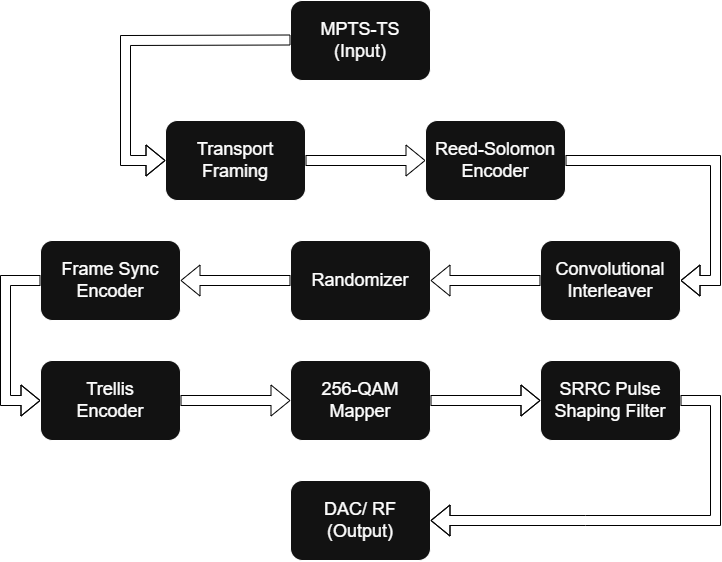
\includegraphics[width=0.64\linewidth]{figures/ch3_j83b_chain.png}
  \caption{J.83B Annex~B downstream processing chain~\cite{ITU_J83}.}
  \label{fig:j83b_chain}
\end{figure}

% ------------------------------------------------------------
\section{DOCSIS 3.0 Downstream Overview}
\label{sec:docsis_overview}

\ac{docsis} 3.0 is the cable industry standard governing broadband
data transmission over \ac{hfc} networks~\cite{DOCSIS3}.
In the downstream direction, from cable headend to \ac{cpe},
\ac{docsis}~3.0 employs \ac{scqam} channels. Each channel
occupies a 6\,MHz bandwidth slot in the North American channel
plan~\cite{SCTE07}.

The downstream channel structure relevant to this work is summarized
in Table~\ref{tab:docsis_params}.

\begin{table}[htbp]
  \caption{DOCSIS 3.0 downstream SC-QAM channel parameters
           (North America)~\cite{DOCSIS3,SCTE07}.}
  \label{tab:docsis_params}
  \centering
  \begin{tabular}{ll}
    \hline
    Parameter           & Value \\
    \hline
    Channel bandwidth   & 6\,MHz \\
    Modulation          & 256-QAM (J.83B Annex~B) \\
    Symbol rate         & 5.360537\,Msym/s \\
    Bits per symbol     & 8 \\
    Information bit rate & 38.81070\,Mbps \\
    % ^ directly from §B.6.1 Table B.3 — citable
    % Raw bit rate (42.884 Mbps = 5.360537×8) and spectral efficiency
    % (≈6.4 bits/s/Hz) are computed values, not stated in standard —
    % omitted from table; include only if derived values section added
    FEC standard        & ITU-T J.83 Annex~B \\
    \hline
  \end{tabular}
\end{table}

A DOCSIS~3.0 downstream system bonds multiple SC-QAM channels to
increase aggregate throughput~\cite{DOCSIS3}.
Each individual channel is independently modulated and passes through
the complete J.83B Annex~B physical layer processing chain described
in this chapter.
The headend \ac{qam} modulator accepts a stream of \ac{mpegts}
packets from the \ac{cmts} and produces
a modulated \ac{rf} signal for distribution over the coaxial plant.
At the subscriber end, a cable modem or set-top box tuner demodulates
the \ac{rf} signal and recovers the \ac{mpegts} byte stream~\cite{DOCSIS3}.

The \ac{qam256} modulation format mandated by J.83B Annex~B~\cite{ITU_J83}
places stringent requirements on the linearity and phase noise
performance of the transmit and receive \ac{rf} chains, and on the
precision of the digital baseband processing blocks described
in the sections that follow~\cite{ITU_J83}.

% ------------------------------------------------------------

\section{J.83B Annex B Standard}
\label{sec:j83b_standard}

ITU-T Recommendation J.83 defines digital multi-programme systems
for television, sound, and data services over cable distribution
networks~\cite{ITU_J83}.
Annex B of the recommendation specifies the physical layer standard
adopted in North America, covering the downstream transmission chain
from MPEG transport stream input to the modulated RF output delivered
over the HFC plant~\cite{ITU_J83,SCTE07}.

The Annex B standard defines a fixed, ordered sequence of processing
stages applied to each MPEG-TS byte stream before modulation.
Table~\ref{tab:j83b_chain_stages} lists each stage in order, together
with the corresponding standard section reference and its role in
the chain.

\begin{table}[htbp]
  \caption{J.83B Annex~B downstream processing chain stages~\cite{ITU_J83}.}
  \label{tab:j83b_chain_stages}
  \centering
  \begin{tabular}{clll}
    \hline
    Stage & Block & Standard Section & Role \\
    \hline
    1 & Transport Framing    & \S B.4     & MPEG-TS packet alignment \\
    2 & Reed-Solomon Encoding & \S B.5.1  & Forward error correction \\
    3 & Convolutional Interleaving & \S B.5.2 & Burst error dispersal \\
    4 & Randomization        & \S B.5.4   & Spectral whitening \\
    5 & Frame Sync Encoding  & \S B.5.3   & Receiver frame lock \\
    6 & Trellis Coding       & \S B.5.5   & Coded modulation \\
    7 & 256-QAM Mapping      & \S B.5.5.5 & Symbol constellation \\
    8 & SRRC Pulse Shaping   & \S B.6.1   & Bandlimited waveform \\
    \hline
  \end{tabular}
\end{table}

Each stage in the chain is described individually in
Sections~\ref{sec:rs_encoding} through~\ref{sec:srrc}.
The remainder of this section provides an overview of the complete
chain and the key system-level parameters that govern its operation.

\paragraph{Transport Framing:}

The chain begins with transport framing, which operates on
MPEG-TS packets of 188 bytes each~\cite{ITU_J83}.
Each packet begins with the standard sync byte \texttt{0x47}~\cite{ITU_J83}.
The framing stage replaces this sync byte in every packet with a
computed parity checksum, derived as the coset of an \ac{fec} parity
check over the preceding 187 payload bytes~\cite{ITU_J83}.
The receiver uses the checksum to detect packet boundaries and
identify packet errors~\cite{ITU_J83}.

\paragraph{Reed-Solomon Encoding:}

\ac{rs} encoding provides the primary \ac{fec}
layer~\cite{ITU_J83}.
The encoder operates on blocks of 122 seven-bit symbols and appends
6 parity symbols to produce a 128-symbol output block~\cite{ITU_J83}.
The code is defined over the Galois field $\mathrm{GF}(2^7)$
and can correct up to 3 symbol errors per block~\cite{ITU_J83}.

\paragraph{Convolutional Interleaving:}

Convolutional interleaving disperses burst errors across multiple
Reed-Solomon blocks so that a single burst affecting several
consecutive bytes at the receiver is spread into correctable
single-byte errors after de-interleaving~\cite{ITU_J83}.
The interleaver is a Forney (convolutional) type with depth
$I = 128$ and increment $J = 1$.

\paragraph{Randomization:}

The randomizer applies a \ac{pn} scrambling sequence to
the interleaved byte stream~\cite{ITU_J83}.
The scrambler operates in $\mathrm{GF}(128)$, initializing its
state to \texttt{0x7F} at each frame boundary and XOR-ing each
7-bit symbol with the \ac{pn} sequence output.
Randomization prevents long runs of identical symbols that would
cause spectral lines in the transmitted signal.

\paragraph{Frame Sync Encoding:}

Frame sync encoding appends a 40-bit trailer to the end of each
FEC frame~\cite{ITU_J83}.
The trailer is packed MSB-first into 7-bit symbols and provides
the receiver with a known pattern for frame boundary detection.

\paragraph{Trellis Coding:}

Trellis coding is applied after frame sync encoding using a 16-state
\ac{bcc} with generator polynomials
$G_1 = 25_8$ and $G_2 = 37_8$~\cite{ITU_J83}.
The \ac{bcc} operates at a punctured rate of 4/5, converting the base
rate 1/2 encoder to produce 5 coded bits for every 4 input
bits~\cite{ITU_J83}.
For \ac{qam256}, the overall trellis coded modulation rate is
19/20~\cite{ITU_J83}, producing 8-bit trellis-coded
words~(C-words) suitable for \ac{qam256} mapping.
A differential precoder is incorporated to resolve phase ambiguity
at the receiver~\cite{ITU_J83}.

\paragraph{256-QAM Symbol Mapping:}

Each 8-bit C-word is mapped to a complex \ac{iq} symbol on the
\ac{qam256} constellation defined by J.83B Figure~B.19~\cite{ITU_J83}.
The output is a stream of complex \ac{iq} samples at the symbol rate
of 5.360537\,Msym/s~\cite{ITU_J83}.
The output is a stream of complex \ac{iq} samples at the symbol rate
of 5.360537\,Msym/s~\cite{ITU_J83}.

\paragraph{SRRC Pulse Shaping:}

The final stage applies \ac{srrc} pulse shaping to the symbol stream.
Table~B.3 of the standard specifies the frequency response as a
\ac{srrc} filter with roll-off $\alpha \approx 0.12$
for \ac{qam256}~\cite{ITU_J83}.
The matched \ac{srrc} filter at the receiver completes the Nyquist
pair, minimizing \ac{isi} at the
sampling instants~\cite{ITU_J83}.
% NOTE: Filter span, samples per symbol, tap count, and output
% sample rate are implementation parameters sourced from
% j83b_srrc_tx.m — NOT stated in the standard.
% These belong in CH-4 (NDA-gated implementation section).
% Do not expand these values in CH-3.

% ------------------------------------------------------------

\section{Reed-Solomon Encoding}
\label{sec:rs_encoding}

\ac{rs} coding forms the outermost layer of the J.83B
\ac{fec} stack, providing block-level error
correction before the data enters the interleaver~\cite{ITU_J83}.
The same \ac{rs} code is used for both 64-QAM and \ac{qam256} operation,
though the \ac{fec} frame format differs between the two modulation
types~\cite{ITU_J83}.

\subsection{Code Definition}

The J.83B \ac{rs} encoder implements a systematic, extended
$(128,\,122)$ \ac{rs} code over the Galois field
$\mathrm{GF}(128) = \mathrm{GF}(2^7)$~\cite{ITU_J83}.
The code corrects up to $t = 3$ symbol errors per \ac{rs} block~\cite{ITU_J83}.
Each symbol is 7 bits wide, matching the field size.

The field is constructed using the primitive polynomial~\cite{ITU_J83}

\begin{equation}
  p(x) = x^7 + x^3 + 1, \quad p(\alpha) = 0
  \label{eq:rs_primitive_poly}
\end{equation}

\noindent where $\alpha$ is the primitive element of
$\mathrm{GF}(128)$.

The generator polynomial is~\cite{ITU_J83}

\begin{equation}
  g(x) = (x - \alpha)(x - \alpha^2)(x - \alpha^3)(x - \alpha^4)
          (x - \alpha^5)
  \label{eq:rs_generator_poly}
\end{equation}

\noindent which expands to

\begin{equation}
  g(x) = x^5 + \alpha^{52}x^4 + \alpha^{116}x^3
             + \alpha^{119}x^2 + \alpha^{61}x + \alpha^{15}
  \label{eq:rs_generator_expanded}
\end{equation}

\subsection{Encoding Procedure}

The encoder accepts a message block of 122 seven-bit symbols,
represented as the message polynomial~\cite{ITU_J83}

\begin{equation}
  m(x) = m_{121}x^{121} + m_{120}x^{120} + \cdots + m_1 x + m_0
  \label{eq:rs_message_poly}
\end{equation}

The message polynomial is multiplied by $x^5$ and divided by
$g(x)$ to produce the remainder~\cite{ITU_J83}

\begin{equation}
  r(x) = r_4 x^4 + r_3 x^3 + r_2 x^2 + r_1 x + r_0
  \label{eq:rs_remainder}
\end{equation}

\noindent These five coefficients constitute the five RS parity
symbols.
The parity symbols are appended to the message to form a 127-symbol code word~\cite{ITU_J83}.

\begin{equation}
  c(x) = m_{121}x^{126} + \cdots + m_0 x^5
        + r_4 x^4 + r_3 x^3 + r_2 x^2 + r_1 x + r_0
  \label{eq:rs_codeword}
\end{equation}

A valid code word has roots at $\alpha^1$ through $\alpha^5$~\cite{ITU_J83}.

\subsection{Extended Parity Symbol}

The J.83B code is extended from $(127,\,121)$ to $(128,\,122)$
by evaluating the 127-symbol code word at the sixth power of
$\alpha$ ~\cite{ITU_J83}

\begin{equation}
  \bar{c} = c(\alpha^6)
  \label{eq:rs_extended_symbol}
\end{equation}

\noindent This extended parity symbol $\bar{c}$ is appended as
the final symbol of the transmitted RS block, yielding the
complete 128-symbol output structure shown in
Table~\ref{tab:rs_block}.

\begin{table}[htbp]
  \caption{J.83B Reed-Solomon block structure~\cite{ITU_J83}.}
  \label{tab:rs_block}
  \centering
  \begin{tabular}{llc}
    \hline
    Symbol positions & Content & Width \\
    \hline
    1 -- 122   & Information symbols ($m_{121}$ \ldots $m_0$) & 7 bits each \\
    123 -- 127 & RS parity symbols ($r_4$ \ldots $r_0$)       & 7 bits each \\
    128        & Extended symbol ($\bar{c} = c(\alpha^6)$)    & 7 bits \\
    \hline
    Total      & 128 symbols                                   & 896 bits \\
    \hline
  \end{tabular}
\end{table}

The parameters of the RS code are summarized in
Table~\ref{tab:rs_params}.

\begin{table}[htbp]
  \caption{J.83B Reed-Solomon code parameters~\cite{ITU_J83}.}
  \label{tab:rs_params}
  \centering
  \begin{tabular}{ll}
    \hline
    Parameter              & Value \\
    \hline
    Code                   & $(128,\,122)$ extended RS \\
    Field                  & $\mathrm{GF}(2^7) = \mathrm{GF}(128)$ \\
    Symbol width           & 7 bits \\
    Information symbols    & 122 per block \\
    Parity symbols         & 5 (RS) $+$ 1 (extended) $= 6$ total \\
    Output block size      & 128 symbols \\
    Correction capability  & $t = 3$ symbol errors per block \\
    \hline
  \end{tabular}
\end{table}

The \ac{rs} encoder output feeds directly into the convolutional
interleaver described in Section~\ref{sec:interleaving}.
The interleaver disperses the 128-symbol \ac{rs} blocks across
multiple frames so that burst channel errors are converted
into correctable single-symbol errors at the \ac{rs} decoder~\cite{ITU_J83}.

% ------------------------------------------------------------
\section{Convolutional Interleaving}
\label{sec:interleaving}

Convolutional interleaving is applied to the \ac{rs}-encoded byte stream
after the encoder and before the randomizer~\cite{ITU_J83}.
Its purpose is to disperse burst channel errors across multiple \ac{rs}
blocks so that a contiguous sequence of corrupted symbols at the receiver
is spread into isolated single-symbol errors after de-interleaving,
keeping the per-block error count within the three-symbol correction
capability of the $(128,\,122)$ \ac{rs} code~\cite{ITU_J83}.

\subsection{Forney Interleaver Structure}

The J.83B interleaver is a Forney convolutional type, operating on
7-bit symbols that match the \ac{rs} field width~\cite{ITU_J83}.
The structure consists of $I$ parallel delay branches, indexed $b = 0, 1, \ldots, I-1$,
with a commutator that cycles through the branches sequentially at the
\ac{rs} symbol rate~\cite{ITU_J83}.
At the start of each \ac{fec} frame the commutator is initialized to
branch~0~\cite{ITU_J83}.

Branch $b$ introduces a delay of~\cite{ITU_J83}

\begin{equation}
  d_b = b \cdot J \quad \text{symbols,} \quad b = 0, 1, \ldots, I-1
  \label{eq:interleaver_branch_delay}
\end{equation}

\noindent so that branch~0 passes symbols with zero delay, branch~1
delays by $J$ symbols, branch~2 by $2J$ symbols, and so on up to
branch $I-1$ which introduces a delay of $(I-1)\cdot J$
symbols.
The de-interleaver at the receiver mirrors this structure, assigning to
branch~$b$ a complementary delay of $(I-1-b)\cdot J$ symbols, so that
the combined round-trip delay is constant at $(I-1)\cdot J$ symbols for
every symbol regardless of which branch it traverses~\cite{ITU_J83}.

The round-trip symbol latency through the interleaver--de-interleaver
pair is therefore

\begin{equation}
  L = I \cdot (I-1) \cdot J \quad \text{symbols.}
  \label{eq:interleaver_latency}
\end{equation}

% [ALT: Block diagram of the J.83B Annex B convolutional interleaver.
%       Input arrives from the Reed-Solomon Encoder as a 7-bit symbol
%       stream and enters an input commutator on the left. The commutator
%       distributes symbols across I parallel delay branches. Branch 1
%       is a direct zero-delay connection. Branch 2 passes through one
%       J-symbol delay register; Branch 3 through two; continuing to
%       Branch I which passes through I-1 registers. An output commutator
%       on the right collects symbols from all branches and passes the
%       interleaved 7-bit stream to the Randomizer.]
\begin{figure}[htbp]
  \centering
  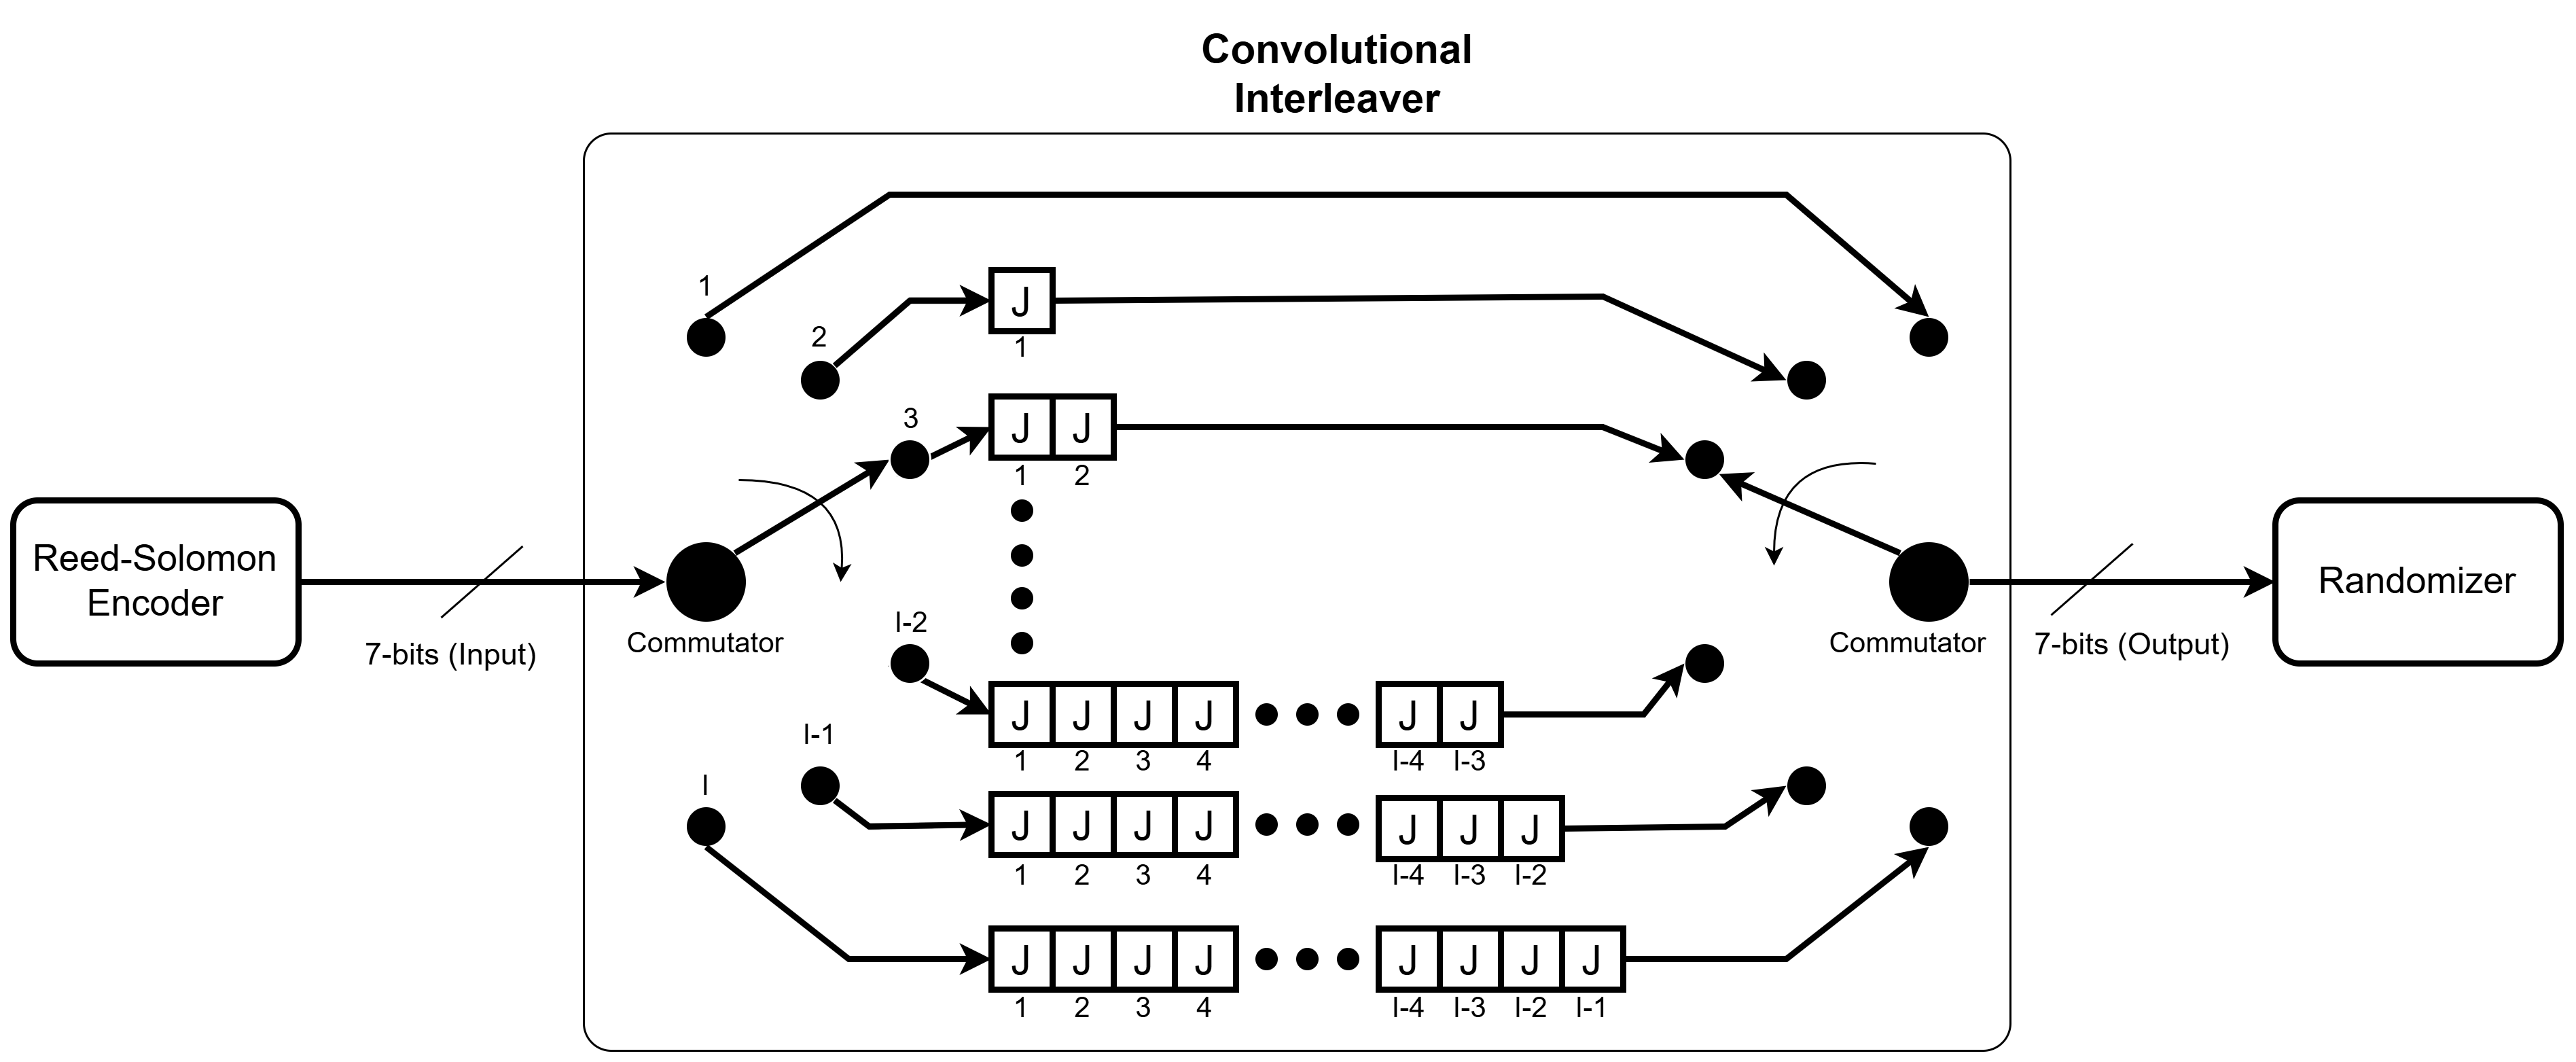
\includegraphics[width=\linewidth]{figures/ch3_interleaver.png}
  \caption{J.83B Annex~B convolutional interleaver structure~\cite{ITU_J83}.
           Branch~$b$ introduces a delay of $b \cdot J$ symbols;
           Branch~1 is a direct connection with zero delay.
           Input commutator cycles at the \ac{rs} symbol rate;
           output feeds the randomizer.}
  \label{fig:interleaver}
\end{figure}

\subsection{Operating Levels and Mode Selection}

J.83B defines two interleaver operating levels~\cite{ITU_J83}.
Level~1 supports a single fixed configuration ($I = 128$, $J = 1$)
and is specified for \ac{docsis} 64-QAM transmission only~\cite{ITU_J83}.
Level~2 extends interleaver support to both 64-QAM and \ac{qam256}
modulation and allows variable interleaving parameters~\cite{ITU_J83}.
A 4-bit in-band control word transmitted during the \ac{fec} frame sync
interval conveys the selected $I$ and $J$ values to the receiver for
the active channel~\cite{ITU_J83}.
Table~\ref{tab:interleaver_modes} lists the defined Level~2 parameter
combinations together with the corresponding burst protection and
latency figures from Table~B.2 of the standard~\cite{ITU_J83}.

\begin{table}[htbp]
  \caption{J.83B Level~2 interleaver parameter options~\cite{ITU_J83}.}
  \label{tab:interleaver_modes}
  \centering
  \begin{tabular}{ccccc}
    \hline
    Control Word & $I$ & $J$ &
      Burst Protection ($\mu$s) &
      Latency, 256-QAM (ms) \\
    \hline
    0001 & 128 & 1 & 66  & 2.8 \\
    0011 &  64 & 2 & 33  & 1.4 \\
    0101 &  32 & 4 & 16  & 0.68 \\
    0111 &  16 & 8 & 8.2 & 0.33 \\
    1001 &   8 & 16 & 4.1 & 0.15 \\
    \hline
  \end{tabular}
\end{table}

The burst protection and latency figures in
Table~\ref{tab:interleaver_modes} exhibit a design trade-off: deeper
interleaving ($I = 128$, $J = 1$) provides greater immunity to
sustained burst noise at the cost of higher end-to-end processing
latency, while shallower configurations reduce latency at the expense
of burst tolerance~\cite{ITU_J83}.

\subsection{Parameters Used in This Work}

This implementation operates in Level~2 mode with control word
\texttt{0001}, corresponding to $I = 128$ branches and increment
$J = 1$ symbol per branch~\cite{ITU_J83}.
This is the maximum-depth configuration and provides the highest burst
protection of the defined Level~2 modes~\cite{ITU_J83}.
Substituting into~\eqref{eq:interleaver_latency}, the round-trip
interleaver--de-interleaver latency is

\begin{equation}
  L = 128 \cdot 127 \cdot 1 = 16{,}256 \quad \text{symbols,}
  \label{eq:interleaver_latency_val}
\end{equation}

\noindent corresponding to a one-way \ac{qam256} channel latency of
2.8\,ms as specified in Table~B.2 of the standard~\cite{ITU_J83}.
The burst protection figure for this mode is
$66\,\mu\mathrm{s}$~\cite{ITU_J83}, which bounds the maximum contiguous
burst duration that the combined interleaver and \ac{rs} decoder can
fully correct.

The interleaved symbol stream feeds directly into the randomizer
described in Section~\ref{sec:randomization}, where a \ac{pn} sequence
is applied for spectral whitening prior to frame sync encoding and
trellis coding~\cite{ITU_J83}.


% ------------------------------------------------------------
\section{Randomization}
\label{sec:randomization}

The randomizer is applied to the interleaved symbol stream after
the convolutional interleaver and before frame sync
encoding~\cite{ITU_J83}.
Its function is to ensure even distribution of symbols across the
\ac{qam256} constellation, which is required for the demodulator
to maintain carrier and timing lock~\cite{ITU_J83}.
Without randomization, long runs of identical symbols produce
spectral lines in the transmitted signal and reduce the effectiveness
of the automatic gain control and phase-locked loop circuits in the
receiver~\cite{ITU_J83}.

\subsection{PN Sequence Generator}

The randomizer XORs each 7-bit interleaved symbol with a
corresponding symbol from a \ac{pn} sequence defined over
$\mathrm{GF}(128) = \mathrm{GF}(2^7)$~\cite{ITU_J83}.
The \ac{pn} sequence is generated by a \ac{lfsr} governed by
the GF(128) recurrence polynomial~\cite{ITU_J83}

\begin{equation}
  f(x) = x^3 + x + \alpha^3
  \label{eq:rand_poly}
\end{equation}

\noindent where $\alpha$ is the primitive element of
$\mathrm{GF}(128)$ satisfying the same reduction polynomial used
by the \ac{rs} encoder~\cite{ITU_J83},

\begin{equation}
  p(x) = x^7 + x^3 + 1.
  \label{eq:rand_reduction_poly}
\end{equation}

The \ac{lfsr} consists of three 7-bit state registers operating
over $\mathrm{GF}(128)$~\cite{ITU_J83}.
At each clock step the register state advances according to
the recurrence in~\eqref{eq:rand_poly}, producing one 7-bit
\ac{pn} output symbol per step.
Each output symbol is bitwise XOR-ed with the corresponding
interleaved data symbol, leaving the 7-bit width of the symbol
stream unchanged~\cite{ITU_J83}.

\subsection{Initialization and Frame Synchronization}

The randomizer is initialized at each \ac{fec} frame
boundary~\cite{ITU_J83}.
Initialization loads all three \ac{lfsr} state registers to the
all-ones state \texttt{0x7F}~\cite{ITU_J83}.
The initialization occurs during the \ac{fec} frame sync trailer
interval; the trailer symbols themselves are therefore not
randomized~\cite{ITU_J83}.
The initialized register state produces the first \ac{pn} output
symbol, which randomizes the first data symbol of the subsequent
\ac{fec} frame~\cite{ITU_J83}.

For \ac{qam256} operation, one \ac{fec} frame consists of
88 \ac{rs} blocks of 128 symbols each, giving a frame data payload
of $88 \times 128 = 11{,}264$ symbols~\cite{ITU_J83}.
The \ac{pn} sequence therefore has a period of 11{,}264 symbols
per frame and is re-initialized at the start of each
frame~\cite{ITU_J83}.

\subsection{Randomizer Parameters}

The randomizer parameters for \ac{qam256} operation are summarized
in Table~\ref{tab:rand_params}.

\begin{table}[htbp]
  \caption{J.83B Annex~B randomizer parameters for
           256-QAM operation~\cite{ITU_J83}.}
  \label{tab:rand_params}
  \centering
  \begin{tabular}{ll}
    \hline
    Parameter              & Value \\
    \hline
    Sequence type          & \ac{lfsr} over $\mathrm{GF}(2^7)$ \\
    Recurrence polynomial  & $f(x) = x^3 + x + \alpha^3$ \\
    Reduction polynomial   & $p(x) = x^7 + x^3 + 1$ \\
    Symbol width           & 7 bits \\
    Initialization state   & \texttt{0x7F} (all ones) \\
    Init trigger           & \ac{fec} frame trailer interval \\
    Operation              & Bitwise XOR per symbol \\
    Sequence period        & $88 \times 128 = 11{,}264$ symbols \\
    \hline
  \end{tabular}
\end{table}

The randomized symbol stream feeds directly into the frame sync
encoder described in Section~\ref{sec:framesync}, where the
\ac{fec} frame trailer is appended and the symbol stream is
unpacked into a serial bit stream for trellis
coding~\cite{ITU_J83}.


% ------------------------------------------------------------
\section{Frame Sync Encoding}
\label{sec:framesync}

Frame sync encoding appends a fixed-pattern trailer to the
randomized symbol stream at the end of each \ac{fec}
frame~\cite{ITU_J83}.
The trailer serves two functions at the receiver: it delineates
the \ac{fec} frame boundary, enabling synchronized \ac{rs}
decoding, de-interleaving, and de-randomization; and it carries
the 4-bit in-band control word that conveys the active interleaver
depth mode to the receiver~\cite{ITU_J83}.
For \ac{qam256}, trellis group boundaries are additionally aligned
to the \ac{fec} frame by the frame sync encoder~\cite{ITU_J83}.

\subsection{FEC Frame Structure}

For \ac{qam256} operation, one \ac{fec} frame consists of 88
\ac{rs} blocks each containing 128 seven-bit symbols~\cite{ITU_J83}.
Each 7-bit symbol is serialized \ac{msb}-first into a contiguous
bit stream, producing~\cite{ITU_J83}

\begin{equation}
  N_\text{data} = 88 \times 128 \times 7 = 78{,}848 \text{ bits}
  \label{eq:fec_data_bits}
\end{equation}

\noindent of data per frame.
The 40-bit sync trailer is appended at the end of the data bit
stream, giving a total frame length of~\cite{ITU_J83}

\begin{equation}
  N_\text{frame} = 78{,}848 + 40 = 78{,}888 \text{ bits}
  \label{eq:fec_frame_bits}
\end{equation}

\noindent which divides exactly into $2076 \times 38$ bits,
corresponding to 2076 trellis groups of 38 input bits
each~\cite{ITU_J83}.
The \ac{rs} block and 7-bit symbol boundaries are aligned to the
end of the \ac{fec} frame~\cite{ITU_J83}.

\begin{table}[htbp]
  \caption{J.83B Annex~B 256-QAM \ac{fec} frame arithmetic~\cite{ITU_J83}.}
  \label{tab:fec_frame_arith}
  \centering
  \begin{tabular}{lr}
    \hline
    Quantity & Value \\
    \hline
    RS blocks per frame           & 88 \\
    Symbols per RS block          & 128 \\
    Bits per symbol (serialized)  & 7 \\
    Data bits per frame           & 78{,}848 \\
    Sync trailer bits             & 40 \\
    Total bits per frame          & 78{,}888 \\
    Trellis groups per frame      & 2{,}076 \\
    Bits per trellis group        & 38 \\
    \hline
  \end{tabular}
\end{table}

\subsection{Sync Trailer Format}

The 40-bit sync trailer is structured as three fields
packed \ac{msb}-first~\cite{ITU_J83}, as shown in
Table~\ref{tab:framesync_trailer}.

\begin{table}[htbp]
  \caption{J.83B Annex~B 256-QAM \ac{fec} frame sync trailer
           structure~\cite{ITU_J83}.}
  \label{tab:framesync_trailer}
  \centering
  \begin{tabular}{clcc}
    \hline
    Field & Content & Width & Value \\
    \hline
    Unique word   & Fixed synchronization pattern & 32 bits
                  & \texttt{71 E8 4D D4}\textsubscript{HEX} \\
    Control word  & Interleaver depth mode        & 4 bits
                  & Level~2 mode code \\
    Reserved      & Set to zero                   & 4 bits
                  & \texttt{0x0} \\
    \hline
    Total         & Sync trailer                  & 40 bits & --- \\
    \hline
  \end{tabular}
\end{table}

The 32-bit unique word \texttt{71 E8 4D D4}\textsubscript{HEX}
is the fixed binary pattern
\begin{center}
\texttt{0111\;0001\;1110\;1000}\\
\texttt{0100\;1101\;1101\;0100}
\end{center}~\cite{ITU_J83}.
The receiver searches for this pattern to detect the \ac{fec}
frame boundary~\cite{ITU_J83}.
The 4-bit control word immediately follows and encodes the active
Level~2 interleaver depth mode as defined in Table~B.2 of the
standard~\cite{ITU_J83}.
The final 4 bits are reserved and set to zero~\cite{ITU_J83}.

The sync trailer is inserted by the encoder and is not
randomized~\cite{ITU_J83}.
The randomizer, described in Section~\ref{sec:randomization}, is
initialized during the trailer interval so that its output is
ready to scramble the first data symbol of the following
frame~\cite{ITU_J83}.

\subsection{Symbol Serialization}

Prior to trellis coding, the frame sync encoder serializes each
7-bit \ac{rs} symbol into individual bits, emitting the most
significant bit first~\cite{ITU_J83}.
The most significant bit of the first \ac{rs} symbol of each
\ac{fec} frame is assigned to the first bit position of the first
non-sync trellis group~\cite{ITU_J83}.
There is no synchronization relationship between the \ac{rs} block
boundaries and \ac{mpegts} packet boundaries; \ac{mpegts}
packet synchronization is obtained independently from \ac{fec}
frame synchronization, keeping the \ac{fec} and transport layers
decoupled~\cite{ITU_J83}.

The serialized bit stream, comprising the 78,848 data bits and the
40-bit trailer (Table~\ref{tab:fec_frame_arith}), feeds directly into the trellis encoder described
in Section~\ref{sec:trellis}~\cite{ITU_J83}.


% ------------------------------------------------------------
\section{Trellis Coding}
\label{sec:trellis}

Trellis coding forms the inner code of the J.83B concatenated
coding scheme~\cite{ITU_J83}.
It introduces redundancy into the transmitted symbol stream to
improve the threshold \ac{snr} by expanding the symbol
constellation without increasing the symbol rate, and is more
precisely termed trellis coded modulation~\cite{ITU_J83}.
For \ac{qam256}, the trellis encoder accepts the serialized bit
stream from the frame sync encoder and produces 8-bit
trellis-coded words, referred to as C-words, that address the
\ac{qam256} constellation mapper~\cite{ITU_J83}.

\subsection{Trellis Group Structure}

The trellis encoder operates on fixed-length groups of input bits
called trellis groups~\cite{ITU_J83}.
For \ac{qam256}, each trellis group contains 38 input bits and
produces 5 output \ac{qam256} symbols, for a total of 40 output
bits per group~\cite{ITU_J83}.

Two types of trellis groups are defined for
\ac{qam256}~\cite{ITU_J83}:

\begin{itemize}
  \item \textbf{Non-sync group:} contains 38 data bits, all
        sourced from the serialized \ac{rs} symbol
        stream~\cite{ITU_J83}.
  \item \textbf{Sync group:} contains 30 data bits and 8 sync
        bits drawn from the \ac{fec} frame sync
        trailer~\cite{ITU_J83}.
        The sync bits occupy only the convolutionally encoded
        bit positions within the group~\cite{ITU_J83}.
\end{itemize}

Since each \ac{fec} frame contains $78{,}888$ bits total (88 \ac{rs}
blocks plus the 40-bit trailer), the frame divides into
$78{,}888 / 38 = 2{,}076$ trellis groups~\cite{ITU_J83}.
Of these, 2{,}071 are non-sync groups and 5 are sync groups;
the 5 sync groups appear at the end of the
frame~\cite{ITU_J83}.

Within each trellis group, the 38 input bits are partitioned by a
data formatter into four streams: the \ac{msb}s of the `A'
symbols, the \ac{msb}s of the `B' symbols, the \ac{lsb}s of
the `A' symbols, and the \ac{lsb}s of the `B'
symbols~\cite{ITU_J83}.
The \ac{msb} streams bypass the convolutional encoder and are
passed directly to the \ac{qam256} mapper
uncoded~\cite{ITU_J83}.
The \ac{lsb} streams are differentially precoded and then
convolutionally encoded before mapping~\cite{ITU_J83}.

\subsection{Binary Convolutional Coder}

The convolutional encoder is a 16-state, non-systematic,
rate~$\frac{1}{2}$ \ac{bcc} with generator
polynomials~\cite{ITU_J83}

\begin{equation}
  G_1(D) = 1 + D^2 + D^4
  \label{eq:bcc_g1}
\end{equation}

\begin{equation}
  G_2(D) = 1 + D + D^2 + D^3 + D^4
  \label{eq:bcc_g2}
\end{equation}

\noindent corresponding to the octal pair $(G_1, G_2) =
(25_8,\,37_8)$~\cite{ITU_J83}.
For each input bit presented to the encoder, two bits are produced
at the output: the $G_1$ output followed by the $G_2$
output~\cite{ITU_J83}.
The commutator is initialized to the $G_1$ position at the
beginning of each trellis group~\cite{ITU_J83}.

Four input bits per trellis group produce 8 convolutionally
encoded bits~\cite{ITU_J83}.
These 8 bits are reduced to 5 by a puncture matrix applied
over the 4-input block~\cite{ITU_J83}

\begin{equation}
  \begin{bmatrix} P_1 \\ P_2 \end{bmatrix}
  =
  \begin{bmatrix} 0 & 0 & 0 & 1 \\ 1 & 1 & 1 & 1 \end{bmatrix}
  \label{eq:bcc_puncture}
\end{equation}

\noindent where $1$ denotes transmission and $0$ denotes suppression.
The puncture matrix converts the rate~$\frac{1}{2}$ encoder to
rate~$\frac{4}{5}$, retaining 5 of the 8 encoded bits per trellis
group~\cite{ITU_J83}.
Two independent \ac{bcc} instances operate in parallel: one
encodes the `A' \ac{lsb} stream producing outputs $U_1$ through
$U_5$, and one encodes the `B' \ac{lsb} stream producing outputs
$V_1$ through $V_5$~\cite{ITU_J83}.

\subsection{Differential Precoder}

Prior to convolutional encoding, the \ac{lsb} streams pass
through a differential precoder that provides 90° rotational
invariance~\cite{ITU_J83}.
Rotational invariance allows the receiver to recover data
correctly following a carrier phase slip without requiring
\ac{fec} resynchronization, since information is carried by the
change in phase rather than its absolute
value~\cite{ITU_J83}.
For \ac{qam256}, the 4th and 8th bits of each C-word are
differentially encoded, corresponding to positions $C_4$ and $C_0$
in the constellation labelling of Figure~B.19 of the
standard~\cite{ITU_J83}.

The differential precoder update equations
are~\cite{ITU_J83}

\begin{equation}
  x_J = W_J \oplus x_{J-1} \oplus Z_J \cdot (x_{J-1} \oplus Y_{J-1})
  \label{eq:precode_x}
\end{equation}

\begin{equation}
  Y_J = Z_J \oplus W_J \oplus Y_{J-1} \oplus Z_J \cdot (x_{J-1} \oplus Y_{J-1})
  \label{eq:precode_y}
\end{equation}

\noindent where $W_J$ and $Z_J$ are the two input bits at step
$J$, $x_J$ and $Y_J$ are the two precoded output bits, $\oplus$
denotes XOR, and $(\cdot)$ denotes the AND
operation~\cite{ITU_J83}.

\subsection{Overall Code Rate and Output}

Each trellis group produces 40 output bits from 38 input bits,
giving an overall trellis coded modulation rate
of~\cite{ITU_J83}

\begin{equation}
  R_\text{TCM} = \frac{38}{40} = \frac{19}{20}
  \label{eq:trellis_rate}
\end{equation}

The 40 output bits per trellis group are packed into 5 eight-bit
C-words, each of which addresses one symbol position in the
\ac{qam256} constellation~\cite{ITU_J83}.
The trellis encoder output feeds directly into the \ac{qam256}
symbol mapper described in
Section~\ref{sec:qam256}~\cite{ITU_J83}.

The trellis coding parameters for \ac{qam256} operation are
summarized in Table~\ref{tab:trellis_params}.

\begin{table}[htbp]
  \caption{J.83B Annex~B trellis coding parameters for
           256-QAM operation~\cite{ITU_J83}.}
  \label{tab:trellis_params}
  \centering
  \begin{tabular}{ll}
    \hline
    Parameter                  & Value \\
    \hline
    Encoder type               & 16-state non-systematic \ac{bcc} \\
    Generator polynomials      & $G_1 = 25_8,\; G_2 = 37_8$ \\
    Base code rate             & $1/2$ \\
    Puncture matrix            & $[P_1;\,P_2] = [0001;\,1111]$ \\
    Punctured code rate        & $4/5$ \\
    Overall \ac{tcm} rate     & $19/20$ \\
    Input bits per group       & 38 \\
    Output symbols per group   & 5 \\
    Output bits per group      & 40 \\
    Trellis groups per frame   & 2{,}076 (2{,}071 non-sync $+$ 5 sync) \\
    C-word width               & 8 bits \\
    \hline
  \end{tabular}
\end{table}


% ------------------------------------------------------------
\section{256-QAM Symbol Mapping}
\label{sec:qam256}

The \ac{qam256} symbol mapper converts the 8-bit C-words
produced by the trellis encoder into complex \ac{iq} baseband
symbols for transmission~\cite{ITU_J83}.
Each C-word addresses a look-up table that returns the complex
symbol coordinates corresponding to that C-word's position on the
\ac{qam256} constellation defined by Figure~B.19 of the
standard~\cite{ITU_J83}.
The mapper output is a stream of complex \ac{iq} samples at the
J.83B symbol rate of 5.360537\,Msym/s, which feeds directly into
the \ac{srrc} pulse shaping filter described in
Section~\ref{sec:srrc}~\cite{ITU_J83}.

\subsection{Constellation Geometry}

The J.83B \ac{qam256} constellation is a square, 256-point array
arranged on a $16 \times 16$ grid in the \ac{iq}
plane~\cite{ITU_J83}.
The in-phase and quadrature axes each carry 16 equally spaced
amplitude levels at odd integer values $\{-15,\,-13,\,\ldots,\,-1,
\,+1,\,\ldots,\,+13,\,+15\}$, giving $16^2 = 256$ distinct symbol
positions~\cite{ITU_J83}.
The constellation is symmetric about both the I and Q axes, and
the minimum Euclidean distance between adjacent symbols is
uniform across the grid~\cite{ITU_J83}.

\subsection{C-Word to Symbol Mapping}

The trellis encoder delivers the coded and uncoded 4-bit `A' and
`B' streams to the mapper, which concatenates them into a single
8-bit C-word with C-bit ordering $C_7 C_6 C_5 C_4\,C_3 C_2 C_1
C_0$ where $C_7$ is the \ac{msb}~\cite{ITU_J83}.
The 8-bit C-word takes values in the range $0$\,--\,$255$ and
uniquely identifies one of the 256 constellation points via the
look-up table defined by Figure~B.19 of the standard~\cite{ITU_J83}.
The mapping is a bijection: every C-word value corresponds to
exactly one symbol position, and every symbol position is
addressed by exactly one C-word~\cite{ITU_J83}.

The differential precoder bits $C_4$ and $C_0$ occupy
the two differentially encoded positions within the C-word, as
noted in Section~\ref{sec:trellis}~\cite{ITU_J83}.
The remaining six C-word bits are passed through uncoded and
carry the \ac{msb} streams directly from the data
formatter~\cite{ITU_J83}.

% NOTE: Gray coding is NOT explicitly stated in the J.83B standard text.
% J83B_FACTS.md flags: "verify from Figure B.19 constellation pattern."
% Do NOT claim Gray coding in this section without Figure B.19 verification.
% This note is for the author; remove before submission.

\subsection{IQ Output and Symbol Rate}

The mapper output is a stream of complex baseband samples of
the form $s_k = I_k + j Q_k$, where $I_k$ and $Q_k$ are the
in-phase and quadrature coordinates of the $k$-th mapped
symbol~\cite{ITU_J83}.
One complex sample is produced per C-word, at a rate equal to the
J.83B symbol rate of 5.360537\,Msym/s~\cite{ITU_J83}.

The \ac{qam256} symbol mapping parameters are summarized in
Table~\ref{tab:qam256_params}.

\begin{table}[htbp]
  \caption{J.83B Annex~B 256-QAM symbol mapping
           parameters~\cite{ITU_J83}.}
  \label{tab:qam256_params}
  \centering
  \begin{tabular}{ll}
    \hline
    Parameter              & Value \\
    \hline
    Constellation          & Square 256-QAM \\
    Grid size              & $16 \times 16$ \\
    Symbol positions       & 256 \\
    I/Q amplitude levels   & $\{-15,\,-13,\,\ldots,\,+13,\,+15\}$ \\
    Input C-word width     & 8 bits ($C_7$\,--\,$C_0$) \\
    Mapping definition     & Figure~B.19, ITU-T J.83 Annex~B \\
    Implementation         & Look-up table (bijection) \\
    Output                 & Complex \ac{iq} symbol stream \\
    Symbol rate            & 5.360537\,Msym/s \\
    \hline
  \end{tabular}
\end{table}


% ------------------------------------------------------------
\section{SRRC Pulse Shaping}
\label{sec:srrc}

\ac{srrc} pulse shaping is the final stage of the J.83B transmit
processing chain, applied to the complex \ac{iq} symbol stream
after \ac{qam256} mapping~\cite{ITU_J83}.
The \ac{srrc} filter bandlimits the symbol stream to fit within
the 6\,MHz channel allocation, controls the spectral shape of the
transmitted signal, and forms one half of the matched filter pair
that minimizes \ac{isi} at the receiver sampling
instants~\cite{ITU_J83}.
The standard refers to this filter as a square-root raised cosine
filter in Table~B.3 and as a Root-Nyquist filter in
\S B.6.2~\cite{ITU_J83}.

\subsection{Nyquist Matched Filter Pair}

The J.83B pulse shaping scheme employs a matched \ac{srrc} filter
pair: an \ac{srrc} filter at the transmitter and an identical
\ac{srrc} filter at the receiver~\cite{ITU_J83}.
The cascade of the transmit and receive \ac{srrc} filters satisfies
the Nyquist \ac{isi} criterion~\cite{proakis_dsp}, producing a
raised cosine overall frequency response

\begin{equation}
  H_\text{RC}(f) = H_\text{TX}(f) \cdot H_\text{RX}(f)
                 = \left| H_\text{SRRC}(f) \right|^2
  \label{eq:srrc_matched}
\end{equation}

\noindent where $H_\text{TX}(f) = H_\text{RX}(f) = H_\text{SRRC}(f)$
are the identical transmit and receive \ac{srrc} frequency
responses~\cite{proakis_dsp}.
The raised cosine response $H_\text{RC}(f)$ has zero crossings at
all non-zero integer multiples of the symbol period $T_s =
1/f_\text{sym}$, ensuring zero \ac{isi} at the receiver sampling
instants when the channel is ideal~\cite{proakis_dsp}.

The \ac{srrc} frequency response is~\cite{proakis_dsp}

\begin{equation}
  H_\text{SRRC}(f) =
  \begin{cases}
    \sqrt{T_s}, & |f| \leq \dfrac{1-\alpha}{2T_s} \\[6pt]
    \sqrt{\dfrac{T_s}{2}\!\left[1 + \cos\!\left(
      \dfrac{\pi T_s}{\alpha}\!\left(|f| - \dfrac{1-\alpha}{2T_s}
      \right)\right)\right]}, &
      \dfrac{1-\alpha}{2T_s} < |f| \leq \dfrac{1+\alpha}{2T_s} \\[6pt]
    0, & |f| > \dfrac{1+\alpha}{2T_s}
  \end{cases}
  \label{eq:srrc_response}
\end{equation}

\noindent where $f_\text{sym} = 1/T_s$ is the symbol rate and
$\alpha$ is the roll-off factor~\cite{proakis_dsp}.
The one-sided occupied bandwidth of the filtered signal is
$(1+\alpha)/(2T_s)$, so the total double-sided bandwidth is
$(1+\alpha) \cdot f_\text{sym}$~\cite{proakis_dsp}.

\subsection{J.83B Filter Specification}

For \ac{qam256}, Table~B.3 of the standard specifies the transmit
filter as a square-root raised cosine with roll-off
factor~\cite{ITU_J83}

\begin{equation}
  \alpha = 0.12 \quad \text{(256-QAM)}
  \label{eq:srrc_alpha}
\end{equation}

\noindent and the symbol rate~\cite{ITU_J83}

\begin{equation}
  f_\text{sym} = 5.360537\,\text{Msym/s} \pm 5\,\text{ppm.}
  \label{eq:srrc_symrate}
\end{equation}

Substituting into the bandwidth expression, the double-sided
occupied bandwidth of the J.83B \ac{qam256} channel
is~\cite{ITU_J83}

\begin{equation}
  B = (1 + \alpha) \cdot f_\text{sym}
    = 1.12 \times 5.360537 \approx 6.004\,\text{MHz}
  \label{eq:srrc_bw}
\end{equation}

\noindent which fits within the 6\,MHz channel slot defined by the
North American channel plan~\cite{ITU_J83,SCTE07}.

\subsection{RF Output Signal Model}

The \ac{rf} modulated output signal is formed by modulating the
\ac{srrc}-filtered baseband \ac{iq} components onto the carrier
frequency $f_c$~\cite{ITU_J83}

\begin{equation}
  s(t) = I(t)\cos(2\pi f_c t) - Q(t)\sin(2\pi f_c t)
  \label{eq:rf_output}
\end{equation}

\noindent where $I(t)$ and $Q(t)$ are the Root-Nyquist filtered
baseband in-phase and quadrature components of the constellation
symbols, and $f_c$ is the \ac{rf} carrier
frequency~\cite{ITU_J83}.

The J.83B \ac{srrc} pulse shaping parameters are summarized in
Table~\ref{tab:srrc_params}.
Filter implementation parameters - including filter span, samples
per symbol, tap count, and output sample rate - are
implementation-specific design choices and are described in
Chapter~4.

\begin{table}[htbp]
  \caption{J.83B Annex~B \ac{srrc} pulse shaping parameters for
           256-QAM operation (standard-sourced)~\cite{ITU_J83}.}
  \label{tab:srrc_params}
  \centering
  \begin{tabular}{ll}
    \hline
    Parameter              & Value \\
    \hline
    Filter type            & Square-root raised cosine (\ac{srrc}) \\
    Standard reference     & \S B.6.1 Table~B.3, \S B.6.2 \\
    Roll-off factor $\alpha$ & 0.12 (256-QAM) \\
    Symbol rate input      & 5.360537\,Msym/s $\pm$ 5\,ppm \\
    Occupied bandwidth     & $\approx 6.004$\,MHz \\
    Channel slot           & 6\,MHz \\
    Matched filter         & TX \ac{srrc} $\times$ RX \ac{srrc} $=$ RC \\
    \ac{isi} at sampling  & Zero (Nyquist criterion, ideal channel) \\
    \hline
  \end{tabular}
\end{table}
% ============================================================
% ch4_implementation.tex
% ANSpect O-EMA · MS Thesis · UTD Electrical Engineering
% \input target — no \documentclass or \begin{document}
% STATUS: NDA-IMPL GATED — see NDA_SCOPE.md
%         Section 4.8 OPEN — all others require handoff + NDA CLEAR
% v1.0  01-Sep-2026  Split from chapters.tex
% ============================================================

% ============================================================
% CHAPTER 4 — IMPLEMENTATION
% STATUS: NDA-IMPL — CHAPTER GATED
%
% GATE REQUIREMENTS (all must be met before any section drafts):
%   1. NDA CLEAR: IMPL [section] received for that section
%   2. Handoff file for that module uploaded in current session
%   3. Content sourced exclusively from handoff file
%   4. nda scrub run on all output before delivery
%
% EXCEPTION: Section 4.8 (Test and Measurement) — OPEN
%   4.8.1 H-Thunder-1 — public product spec
%   4.8.2 HDHomeRun    — public product
%   4.8.3 Spectrum analysis — general methodology
% ============================================================

\chapter{Implementation}
\label{ch:implementation}
% [NDA-IMPL] — chapter-level gate active
% TODO: Chapter intro paragraph — structural overview only
%   - High-level system block: PS + PL + RFDC + RF front-end
%   - No architecture detail until NDA CLEAR: IMPL [4.1] received
%   - Reference PYNQ framework existence (no internals)
 
% ------------------------------------------------------------
\section{System Architecture Overview}
\label{sec:sys_arch}
% [NDA-IMPL] — BLOCKED
% TODO: Draft requires NDA CLEAR: IMPL [4.1] + handoff upload
%   - Top-level system diagram
%   - PS/PL partition overview
%   - Data flow: UDP RX → TX chain → DAC → RF → ADC → RX chain → output
%   - No AXI register map, no overlay internals without clearance
\clearpage  
% ------------------------------------------------------------
\section{Processing System}
\label{sec:ps}
% [NDA-IMPL] — BLOCKED
% TODO: Draft requires NDA CLEAR: IMPL [4.2] + handoff upload
%   - PS subsystem structural overview only
%   - No Python driver detail, no DMA control code without clearance

\subsection{UDP/GigE RX}
\label{subsec:ps_udp_rx}
% [NDA-IMPL] — BLOCKED (PS-01)
% TODO: Requires NDA CLEAR: IMPL [4.2.1] + handoff for PS-01

\subsection{TX Chain}
\label{subsec:ps_tx_chain}
% [NDA-IMPL] — BLOCKED (PS-02)
% TODO: Requires NDA CLEAR: IMPL [4.2.2] + handoff for PS-02

\subsection{DMA Control}
\label{subsec:ps_dma_control}
% [NDA-IMPL] — BLOCKED (PS-03, PS-05)
% TODO: Requires NDA CLEAR: IMPL [4.2.3] + handoff for PS-03/PS-05
\clearpage  
% ------------------------------------------------------------
\section{Programmable Logic: TX Chain}
\label{sec:pl_tx}
% [NDA-IMPL] — BLOCKED
% TODO: Section intro requires NDA CLEAR: IMPL [4.3] + handoff
%   - PL-01 through PL-12 — one subsection each
%   - PL-10 (SD-FEC LDPC) also touches [NDA-ALGO] boundary —
%     see subsection note below

\subsection{PL-01: AXI DMA MM2S}
\label{subsec:pl01}
% [NDA-IMPL] — BLOCKED
% TODO: Requires NDA CLEAR: IMPL [4.3.1] + handoff for PL-01

\subsection{PL-02: Transport Framing}
\label{subsec:pl02}
% [NDA-IMPL] — BLOCKED
% TODO: Requires NDA CLEAR: IMPL [4.3.2] + handoff for PL-02

\subsection{PL-03: Reed-Solomon Encoder}
\label{subsec:pl03}
% [NDA-IMPL] — BLOCKED
% TODO: Requires NDA CLEAR: IMPL [4.3.3] + handoff for PL-03

\subsection{PL-04: Convolutional Interleaver}
\label{subsec:pl04}
% [NDA-IMPL] — BLOCKED
% TODO: Requires NDA CLEAR: IMPL [4.3.4] + handoff for PL-04

\subsection{PL-05: Randomizer}
\label{subsec:pl05}
% [NDA-IMPL] — BLOCKED
% TODO: Requires NDA CLEAR: IMPL [4.3.5] + handoff for PL-05

\subsection{PL-06: Frame Sync Encoder}
\label{subsec:pl06}
% [NDA-IMPL] — BLOCKED
% TODO: Requires NDA CLEAR: IMPL [4.3.6] + handoff for PL-06

\subsection{PL-07: Trellis Encoder}
\label{subsec:pl07}
% [NDA-IMPL] — BLOCKED
% TODO: Requires NDA CLEAR: IMPL [4.3.7] + handoff for PL-07

\subsection{PL-08: QAM-256 Mapper}
\label{subsec:pl08}
% [NDA-IMPL] — BLOCKED
% TODO: Requires NDA CLEAR: IMPL [4.3.8] + handoff for PL-08

\subsection{PL-09: SRRC FIR TX}
\label{subsec:pl09}
% [NDA-IMPL] — BLOCKED
% TODO: Requires NDA CLEAR: IMPL [4.3.9] + handoff for PL-09

\subsection{PL-10: SD-FEC LDPC}
\label{subsec:pl10}
% [NDA-IMPL] — BLOCKED
% [NDA-ALGO] — LDPC interaction with O-EMA overlay
%              PERMANENTLY BLOCKED — never draftable
% TODO: Structural existence may be acknowledged only
%   - Internal algorithm: hard block, do not draft or paraphrase
%   - Requires NDA CLEAR: IMPL [4.3.10] for structural frame only

\subsection{PL-11: Register File RTL}
\label{subsec:pl11}
% [NDA-IMPL] — BLOCKED
% TODO: Requires NDA CLEAR: IMPL [4.3.11] + handoff for PL-11
%   - AXI-Lite register map is NDA-IMPL — do not include offsets
%     or field definitions without explicit clearance

\subsection{PL-12: IQ Combiner}
\label{subsec:pl12}
% [NDA-IMPL] — BLOCKED
% TODO: Requires NDA CLEAR: IMPL [4.3.12] + handoff for PL-12
\clearpage  
% ------------------------------------------------------------
\section{Programmable Logic: RX Chain}
\label{sec:pl_rx}
% [NDA-IMPL] — BLOCKED
% TODO: Section intro requires NDA CLEAR: IMPL [4.4] + handoff
%   - PL-13 through PL-23 — one subsection each

\subsection{PL-13: SRRC FIR RX}
\label{subsec:pl13}
% [NDA-IMPL] — BLOCKED
% TODO: Requires NDA CLEAR: IMPL [4.4.1] + handoff for PL-13

\subsection{PL-14: Symbol Timing Recovery}
\label{subsec:pl14}
% [NDA-IMPL] — BLOCKED
% TODO: Requires NDA CLEAR: IMPL [4.4.2] + handoff for PL-14

\subsection{PL-15: Carrier and Phase Recovery}
\label{subsec:pl15}
% [NDA-IMPL] — BLOCKED
% TODO: Requires NDA CLEAR: IMPL [4.4.3] + handoff for PL-15

\subsection{PL-16: QAM-256 Demapper}
\label{subsec:pl16}
% [NDA-IMPL] — BLOCKED
% TODO: Requires NDA CLEAR: IMPL [4.4.4] + handoff for PL-16

\subsection{PL-17: Trellis Decoder}
\label{subsec:pl17}
% [NDA-IMPL] — BLOCKED
% TODO: Requires NDA CLEAR: IMPL [4.4.5] + handoff for PL-17

\subsection{PL-18: Frame Sync Detection}
\label{subsec:pl18}
% [NDA-IMPL] — BLOCKED
% TODO: Requires NDA CLEAR: IMPL [4.4.6] + handoff for PL-18

\subsection{PL-19: De-Randomizer}
\label{subsec:pl19}
% [NDA-IMPL] — BLOCKED
% TODO: Requires NDA CLEAR: IMPL [4.4.7] + handoff for PL-19

\subsection{PL-20: De-Interleaver}
\label{subsec:pl20}
% [NDA-IMPL] — BLOCKED
% TODO: Requires NDA CLEAR: IMPL [4.4.8] + handoff for PL-20

\subsection{PL-21: Reed-Solomon Decoder}
\label{subsec:pl21}
% [NDA-IMPL] — BLOCKED
% TODO: Requires NDA CLEAR: IMPL [4.4.9] + handoff for PL-21

\subsection{PL-22: Transport Framing RX}
\label{subsec:pl22}
% [NDA-IMPL] — BLOCKED
% TODO: Requires NDA CLEAR: IMPL [4.4.10] + handoff for PL-22

\subsection{PL-23: AXI DMA S2MM}
\label{subsec:pl23}
% [NDA-IMPL] — BLOCKED
% TODO: Requires NDA CLEAR: IMPL [4.4.11] + handoff for PL-23
\clearpage  
% ------------------------------------------------------------
\section{RF Data Converter}
\label{sec:rfdc}
% [NDA-IMPL] — BLOCKED
% TODO: Section intro requires NDA CLEAR: IMPL [4.5] + handoff
%   - Existence of RFDC block may be stated (public IP)
%   - Tile configuration parameters: NDA-IMPL — no detail without clearance

\subsection{DAC: Tile 228}
\label{subsec:dac_tile228}
% [NDA-IMPL] — BLOCKED (RFDC-01)
% TODO: Requires NDA CLEAR: IMPL [4.5.1] + handoff
%   - Tile/channel configuration: NDA-IMPL
%   - NCO, interpolation settings: NDA-IMPL

\subsection{ADC: Tile 224}
\label{subsec:adc_tile224}
% [NDA-IMPL] — BLOCKED (RFDC-02)
% TODO: Requires NDA CLEAR: IMPL [4.5.2] + handoff
%   - Tile/channel configuration: NDA-IMPL
\clearpage  
% ------------------------------------------------------------
\section{RF Front-End}
\label{sec:rf_frontend}
% [NDA-IMPL] — BLOCKED
% TODO: Section intro requires NDA CLEAR: IMPL [4.6] + handoff

\subsection{TX Path}
\label{subsec:rf_tx}
% [NDA-IMPL] — BLOCKED (RF-01)
% TODO: Requires NDA CLEAR: IMPL [4.6.1] + handoff
%   - DAC balun + SMA TX path

\subsection{RX Path}
\label{subsec:rf_rx}
% [NDA-IMPL] — BLOCKED (RF-02)
% TODO: Requires NDA CLEAR: IMPL [4.6.2] + handoff
%   - ADC balun + SMA RX path
\clearpage  
% ------------------------------------------------------------
\section{Clocking Subsystem}
\label{sec:clocking}
% [NDA-IMPL] — BLOCKED
% TODO: Section intro requires NDA CLEAR: IMPL [4.7] + handoff
%   - Clock chip existence may be stated (public component)
%   - Register settings: NDA-IMPL — no detail without clearance

\subsection{LMK04828}
\label{subsec:lmk04828}
% [NDA-IMPL] — BLOCKED (EXT-01)
% TODO: Requires NDA CLEAR: IMPL [4.7.1] + handoff
%   - Clock distribution chip — register configuration: NDA-IMPL

\subsection{LMX2594}
\label{subsec:lmx2594}
% [NDA-IMPL] — BLOCKED (EXT-02)
% TODO: Requires NDA CLEAR: IMPL [4.7.2] + handoff
%   - PLL/VCO chip — register configuration: NDA-IMPL

\subsection{xrfclk API}
\label{subsec:xrfclk}
% [NDA-IMPL] — BLOCKED (EXT-03)
% TODO: Requires NDA CLEAR: IMPL [4.7.3] + handoff
%   - Xilinx xrfclk Python API — usage detail: NDA-IMPL
\clearpage  
% ------------------------------------------------------------
\section{Test and Measurement}
\label{sec:test_measurement}
% STATUS: OPEN — all subsections freely draftable from public specs
% TODO: Section intro paragraph
%   - Overview of test setup: source → DUT → sink + spectrum
%   - Loopback topology description

\subsection{H-Thunder-1 Reference Signal}
\label{subsec:hthunder}
% STATUS: OPEN — public product spec
% TODO:
%   - H-Thunder-1 J.83B / 256-QAM reference signal generator
%   - Role: known-good J.83B signal source for RX validation
%   - Public product specification detail
%   - Cite product datasheet \cite{NEEDED} % [CITE NEEDED]

\subsection{HDHomeRun: Source and Sink}
\label{subsec:hdhomerun}
% STATUS: OPEN — public product (EXT-04, EXT-05)
% TODO:
%   - HDHomeRun \#1 role: MPEG-TS source over GigE (TX path input)
%   - HDHomeRun \#2 role: MPEG-TS sink over GigE (RX path output)
%   - Public product — cite product page \cite{NEEDED} % [CITE NEEDED]

\subsection{Spectrum Analysis}
\label{subsec:spectrum_analysis}
% STATUS: OPEN — general methodology
% TODO:
%   - Spectrum analyzer role in RF output validation
%   - Measurements performed: channel power, spectral shape,
%     occupied bandwidth, noise floor
%   - General methodology — no proprietary test vector data
\clearpage  
% ------------------------------------------------------------
\section{Verification and Results}
\label{sec:verification}
% [NDA-IMPL] — BLOCKED
% TODO: Section intro requires NDA CLEAR: IMPL [4.9] + handoff
%   - Stage map existence may be referenced (public README portion)
%   - Test vector details: NDA-IMPL

\subsection{Test Vectors}
\label{subsec:test_vectors}
% [NDA-IMPL] — BLOCKED (partially public stage map only)
% TODO: Requires NDA CLEAR: IMPL [4.9.1] + handoff
%   - Stage boundary file names (public): stage0–stage8
%   - File formats (public): uint8 / int16 per stage
%   - Internal content and mismatch analysis: NDA-IMPL

\subsection{Loopback Validation}
\label{subsec:loopback}
% [NDA-IMPL] — BLOCKED
% TODO: Requires NDA CLEAR: IMPL [4.9.2] + handoff
%   - Loopback path topology (structural) may be described after clearance
%   - BER / EVM / verification results: NDA-IMPL

% ============================================================
% ch5_conclusion.tex
% ANSpect O-EMA · MS Thesis · UTD Electrical Engineering
% \input target — no \documentclass or \begin{document}
% STATUS: SKELETON — run 'expand CH-5.X' to flesh out
% v1.0  01-Sep-2026  Split from chapters.tex
% ============================================================

% ============================================================
% CHAPTER 5 — CONCLUSION AND FUTURE WORK
% STATUS: OPEN
% ============================================================

\chapter{Conclusion and Future Work}
\label{ch:conclusion}
% TODO:
%   - Brief synthesis paragraph linking CH-1 problem to outcome
%   - Frame the two sections below

% ------------------------------------------------------------
\section{Summary of Contributions}
\label{sec:contributions_summary}
% TODO:
%   - Restate contributions from Section~\ref{sec:contributions}
%     in past tense with outcome framing
%   Contribution 1: manual SystemVerilog RTL — J.83B Annex B
%     full TX+RX chain — outcome of HDL Coder evaluation
%   Contribution 2: [NDA-TITLE system] — stated generically
%   - Assessment of verification results (high level only;
%     detail deferred to CH-4.9 after NDA clearance)

% ------------------------------------------------------------
\section{Future Work}
\label{sec:future_work}
% TODO:
%   - Enumerate open research directions
%   Candidate directions (do not invent — confirm with advisor):
%   - OFDM / DOCSIS 3.1 SC-FDE extension
%   - Multi-channel concurrent operation on RFSoC 4x2
%   - Real-time MPEG-TS throughput benchmarking
%   - Additional FEC modes or constellation orders
%   - HDL Coder re-evaluation with updated toolchain version
%   - Open-source release and reproducibility packaging

% ------------------------------------------------------------
% BACK MATTER
% ------------------------------------------------------------

% Appendices — none planned; uncomment if added
% \appendix
% \chapter*{Appendix Title}
% % TODO: appendix content

% References — REFERENCES heading auto-generated by thesisbib
\begin{thesisbib}
  \setlength{\bibsep}{12pt plus 1pt minus 1pt}
  \bibliography{references}    % references.bib
\end{thesisbib}

% Biographical Sketch
\begin{biosketch}
  % TODO: third-person biographical sketch
  % May include: education, degrees, publications, experience
  % No \section commands inside biosketch environment
  Sathwik Sudhindranath received the B.E.\ degree in Electronics
  and Communication Engineering from Visvesvaraya Technological
  University, India, in 2021. He is currently pursuing the M.S.\
  degree in Electrical Engineering with a concentration in
  Computing Systems at The University of Texas at Dallas,
  Richardson, Texas, expected December 2026.
  % TODO: add publications, industry experience, or awards if any
\end{biosketch}

% Curriculum Vitae — pages unnumbered, listed in TOC
\begin{vita}
  % TODO: CV content
  % No special formatting requirements
  % External CV pages may be substituted at print time
  % (must still issue \begin{vita}...\end{vita} for TOC entry)
\end{vita}

\end{document}